% =====================================================================================================
%  Defence talk: "When can an automatic answer be trusted?"  (Brhanu Atsbaha, University of Hildesheim)
%  Build:   cd presentation && ~/.local/bin/tectonic -X compile defence_talk.tex
%  Every figure on these slides is taken from the thesis (thesis_v4.pdf) or its result files.
% =====================================================================================================
\documentclass[aspectratio=169,10pt]{beamer}

% ---------- fonts and packages ----------
\usepackage[sfdefault,lining]{FiraSans}
\usepackage{amsmath,amssymb}
\usepackage{booktabs,array,tabularx,colortbl}
\renewcommand{\tabularxcolumn}[1]{m{#1}}
\usepackage{tikz}
\usetikzlibrary{positioning,arrows.meta,fit,backgrounds,calc,shapes.geometric,shapes.misc,decorations.pathreplacing}
\usepackage{pgfplots}\pgfplotsset{compat=1.18,every axis/.append style={tick label style={font=\scriptsize},label style={font=\scriptsize}},
  /pgf/number format/.cd,fixed,precision=3,1000 sep={{{,}}}}
\usepackage[most]{tcolorbox}
\graphicspath{{../latex_assets/}{defence_assets/}{images/}}

% ---------- colours: one meaning each, used in every diagram ----------
\definecolor{ink}{HTML}{1F2933}
\definecolor{navy}{HTML}{1E3A5F}
\definecolor{muted}{HTML}{6B7280}
\definecolor{soft}{HTML}{F3F4F6}
\definecolor{line}{HTML}{D1D5DB}
\definecolor{agent}{HTML}{2F6FAE}     % the three agents
\definecolor{agentbg}{HTML}{E8F0F9}
\definecolor{mapc}{HTML}{7B5EA7}      % learned mappings / probabilities
\definecolor{mapbg}{HTML}{F0EBF7}
\definecolor{risk}{HTML}{C8711E}      % conformal risk control
\definecolor{riskbg}{HTML}{FBF0E4}
\definecolor{okc}{HTML}{2E7D4F}       % approved automatically
\definecolor{okbg}{HTML}{E6F4EC}
\definecolor{pers}{HTML}{B83A3A}      % a person checks
\definecolor{persbg}{HTML}{FBEAEA}
\definecolor{oldc}{HTML}{8A6D3B}      % the first (deployed) design
\definecolor{oldbg}{HTML}{F5EFE3}
\definecolor{tiertwo}{HTML}{4B5563}   % Tier 2 helpers
\definecolor{tiertwobg}{HTML}{EEF0F2}

% ---------- beamer look ----------
\setbeamertemplate{navigation symbols}{}
\setbeamercolor{normal text}{fg=ink,bg=white}
\setbeamercolor{structure}{fg=navy}
\setbeamercolor{alerted text}{fg=pers}
\setbeamerfont{frametitle}{size=\large,series=\bfseries}
\setbeamersize{text margin left=0.55cm,text margin right=0.55cm}
\setbeamertemplate{itemize item}{\color{navy}\raisebox{0.15ex}{\scalebox{0.8}{$\blacktriangleright$}}}
\setbeamertemplate{itemize subitem}{\color{muted}--}
\setbeamertemplate{enumerate item}{\color{navy}\bfseries\insertenumlabel.}
\setlength{\leftmargini}{1.2em}

\setbeamertemplate{frametitle}{%
  \vskip4pt
  \ifx\insertsection\empty\else{\tiny\color{muted}\MakeUppercase{\insertsection}}\par\vskip0pt\fi
  {\usebeamerfont{frametitle}\color{navy}\insertframetitle}\par
  \vskip1pt{\color{line}\rule{\linewidth}{0.5pt}}\vskip-2pt%
}
\setbeamertemplate{footline}{%
  \vskip0.42cm
  \begin{tikzpicture}[remember picture,overlay]
    \fill[line] (current page.south west) ++(0,0.22) rectangle ++(\paperwidth,0.05);
    \pgfmathsetmacro{\progress}{min(1,\insertframenumber/max(1,\inserttotalframenumber))}
    \fill[navy] (current page.south west) ++(0,0.22) rectangle ++({\progress*\paperwidth},0.05);
    \node[anchor=south west,font=\tiny,text=muted] at ($(current page.south west)+(0.35,0.0)$) {Brhanu Atsbaha \,·\, When can an automatic answer be trusted?};
    \node[anchor=south east,font=\tiny,text=muted] at ($(current page.south east)+(-0.35,0.0)$) {\insertframenumber\,/\,\inserttotalframenumber};
  \end{tikzpicture}}

% part divider with the road map
\AtBeginSection{\ifnum\value{section}<7%
  \begin{frame}[plain,noframenumbering]
  \centering\vspace*{1.2cm}
  {\small\color{muted}PART \thesection\ OF 6}\par\vspace{2pt}
  {\Huge\bfseries\color{navy}\insertsection}\par\vspace{1.0cm}
  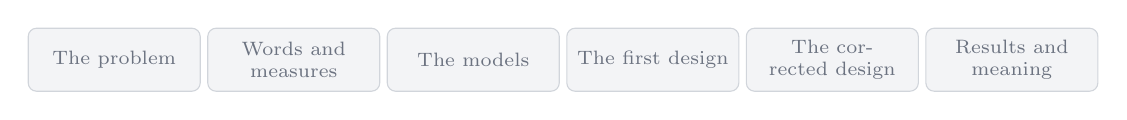
\begin{tikzpicture}
    \foreach \n [count=\i] in {The problem,Words and measures,The models,The first design,The corrected design,Results and meaning}{
      \ifnum\i=\thesection
        \node[draw=navy,fill=navy,text=white,rounded corners=3pt,minimum width=2.1cm,minimum height=0.8cm,font=\scriptsize\bfseries,align=center,text width=1.95cm] at (\i*2.28,0) {\n};
      \else
        \node[draw=line,fill=soft,text=muted,rounded corners=3pt,minimum width=2.1cm,minimum height=0.8cm,font=\scriptsize,align=center,text width=1.95cm] at (\i*2.28,0) {\n};
      \fi}
  \end{tikzpicture}
  \end{frame}\fi}

% ---------- boxes ----------
\newtcolorbox{keybox}[1][]{enhanced,colback=navy!5,colframe=navy,boxrule=0pt,leftrule=3pt,arc=2pt,
  left=6pt,right=6pt,top=4pt,bottom=4pt,fontupper=\small\raggedright,#1}
\newcommand{\defboxfont}{\footnotesize}
\newtcolorbox{defbox}[2][]{enhanced,colback=white,colframe=line,boxrule=0.6pt,arc=3pt,
  title={#2},coltitle=navy,colbacktitle=soft,fonttitle=\small\bfseries,left=5pt,right=5pt,top=3pt,bottom=3pt,
  fontupper=\defboxfont\raggedright,toptitle=1pt,bottomtitle=1pt,#1}
\newtcolorbox{exbox}[1][]{enhanced,colback=okbg,colframe=okc,boxrule=0pt,leftrule=3pt,arc=2pt,
  left=6pt,right=6pt,top=4pt,bottom=4pt,fontupper=\small\raggedright,title={Example},coltitle=okc,colbacktitle=okbg,
  fonttitle=\scriptsize\bfseries,attach title to upper={\ \ },#1}
\newcommand{\relcard}[4]{%
  \begin{tcolorbox}[enhanced,colback=white,colframe=line,boxrule=0.6pt,arc=3pt,left=6pt,right=6pt,top=4pt,bottom=5pt,
    title={#1},coltitle=navy,colbacktitle=soft,fonttitle=\small\bfseries,halign title=flush left,toptitle=2pt,bottomtitle=2pt,fontupper=\footnotesize\raggedright]
  {\scriptsize\color{muted}#2}\par\vspace{3pt}
  {\scriptsize\bfseries\color{muted}WHAT IT SHOWED}\par\vspace{1pt}#3\par\vspace{4pt}
  {\color{line}\rule{\linewidth}{0.5pt}}\par\vspace{3pt}
  {\scriptsize\bfseries\color{navy}WHAT THIS THESIS ADDS}\par\vspace{1pt}{\color{navy}#4}
  \end{tcolorbox}}
\newcommand{\takeaway}[1]{\vfill\begin{keybox}#1\end{keybox}}
\newcommand{\stepn}[1]{{\setlength{\fboxsep}{1.3pt}\colorbox{navy}{\color{white}\bfseries\scriptsize\,#1\,}}}
\newcommand{\yes}[1]{{\color{okc}\bfseries #1}}
\newcommand{\no}[1]{{\color{pers}\bfseries #1}}

% ---------- TikZ styles ----------
\tikzset{
  >={Stealth[length=2mm]},
  box/.style={draw=line,rounded corners=3pt,align=center,inner sep=4pt,fill=white,font=\footnotesize},
  agentb/.style={box,draw=agent,fill=agentbg,minimum width=2.9cm,minimum height=1.05cm},
  mapb/.style={box,draw=mapc,fill=mapbg},
  riskb/.style={box,draw=risk,fill=riskbg},
  okb/.style={box,draw=okc,fill=okbg},
  persb/.style={box,draw=pers,fill=persbg},
  oldb/.style={box,draw=oldc,fill=oldbg},
  greyb/.style={box,draw=tiertwo!60,fill=tiertwobg,text=tiertwo},
  arr/.style={->,thick,color=muted},
  dashedarr/.style={->,thick,dashed,color=muted!70},
  io/.style={font=\scriptsize\bfseries,text=muted},
}



\title{When Can an Automatic Answer Be Trusted?}
\subtitle{Confidence, Not Disagreement, Under a Risk Promise for Historical Illustrations}
\author{Brhanu Atsbaha}
\institute{Master Thesis \,·\, International Master in Data Analytics \,·\, University of Hildesheim\\[2pt]First advisor: Prof.\ Dr.\ Thomas Mandl \,·\, Second advisor: Shereen Elsayed}
\date{Defence, 10 December 2026}

\begin{document}

% =====================================================================================================
\begin{frame}[plain,noframenumbering]
\begin{tikzpicture}[remember picture,overlay]
  \fill[navy] (current page.north west) rectangle ($(current page.north east)+(0,-0.35)$);
  \fill[soft] ($(current page.south west)+(0,0)$) rectangle ($(current page.south east)+(0,2.0)$);
\end{tikzpicture}
\vspace{0.9cm}
{\small\color{muted}MULTI AGENT SYSTEMS FOR IMAGE ANALYSIS: OBJECT AND COMPLEX SCENE DETECTION}\par\vspace{6pt}
{\fontsize{26}{30}\selectfont\bfseries\color{navy}\inserttitle}\par\vspace{6pt}
{\large\color{ink}\insertsubtitle}\par\vspace{0.9cm}
{\bfseries\insertauthor}\par\vspace{2pt}
{\small\color{muted}\insertinstitute}\par\vspace{10pt}
{\small\color{muted}\insertdate}
\note{Good morning. My thesis asks one question about a system that labels pictures in a historical archive: which of its answers can be used without a person checking them? I will show the archive, the models, the first design and why it failed, the corrected design, and what the results allow us to claim.}
\end{frame}


% =====================================================================================================
\section{The problem}

\begin{frame}{The archive: 12,110 illustrations from historical books}
\begin{columns}[T,onlytextwidth]
\column{0.58\textwidth}
\centering
\begin{tikzpicture}
\node[inner sep=0] (a) {\includegraphics[height=2.35cm]{class_family.jpg}};
\node[inner sep=0,right=2mm of a] (b) {\includegraphics[height=2.35cm]{class_landscape.jpg}};
\node[inner sep=0,below=2mm of a.south west,anchor=north west] (c) {\includegraphics[height=2.35cm]{class_playing.jpg}};
\node[inner sep=0,right=2mm of c] (d) {\includegraphics[height=2.35cm]{none_sheet_music.jpg}};
\node[inner sep=0,right=2mm of d] (e) {\includegraphics[height=2.35cm]{none_ornament.jpg}};
\end{tikzpicture}
\column{0.40\textwidth}
\small
\begin{itemize}\setlength\itemsep{4pt}
\item Digitised historical books (Colibri collection): every illustration is cut from its page and becomes one \textbf{picture}.
\item Pictures are old prints: line drawings, engravings, stains, faded ink. Modern models were trained on photos.
\item Not every picture shows a scene: sheet music, ornaments, maps and text pages are pictures too.
\end{itemize}
\vspace{2pt}
{\footnotesize\begin{tabular}{@{}l r@{}}
\toprule
All pictures & 12,110\\
Labelled pool (scene or not) & 1,250\\
\quad from & 550 books\\
With hand-drawn boxes & 300\\
\bottomrule
\end{tabular}}
\end{columns}
\note{The data: 12,110 illustrations from digitised historical books. They are prints, not photographs, which is exactly where modern models are weakest. A labelled pool of 1,250 pictures from 550 books is used for learning and testing; 300 pictures have boxes drawn by hand for the object tasks.}
\end{frame}

\begin{frame}{Two tasks, fixed at the start}
\begin{columns}[T,onlytextwidth]
\column{0.60\textwidth}
\textbf{\color{navy}Task 1 \,·\, Which scene does a picture show?}\par{\footnotesize\color{muted}one of five classes, or ``no scene''}\par\vspace{4pt}
\centering
\setlength{\tabcolsep}{2pt}
\begin{tabular}{ccc}
\includegraphics[height=1.3cm]{class_teaching.jpg}&
\includegraphics[height=1.3cm]{class_family.jpg}&
\includegraphics[height=1.3cm]{class_playing.jpg}\\[-1pt]
\scriptsize teaching&\scriptsize family&\scriptsize playing\\[2pt]
\includegraphics[height=1.3cm]{class_landscape.jpg}&
\includegraphics[height=1.3cm]{class_drawing.jpg}&
\includegraphics[height=1.3cm]{none_sheet_music.jpg}\\[-1pt]
\scriptsize landscape&\scriptsize drawing&\scriptsize no scene
\end{tabular}
\par\vspace{3pt}\raggedright\footnotesize
First level: is there a scene \emph{at all}? (yes / no). ``Drawing'' = figurative, but none of the other four.
\column{0.37\textwidth}
\textbf{\color{navy}Task 2 \,·\, Which objects are in it?}\par\vspace{6pt}
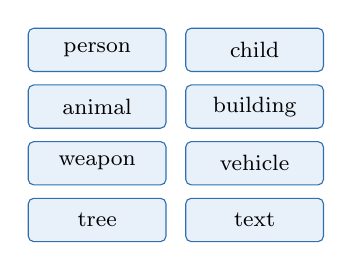
\begin{tikzpicture}[o/.style={draw=agent,fill=agentbg,rounded corners=2pt,font=\footnotesize,minimum width=1.75cm,minimum height=0.55cm}]
\foreach \n [count=\i from 0] in {person,child,animal,building,weapon,vehicle,tree,text}{
  \pgfmathtruncatemacro{\r}{\i/2}\pgfmathtruncatemacro{\c}{mod(\i,2)}
  \node[o] at (\c*2.0,-\r*0.72) {\n};}
\end{tikzpicture}
\par\vspace{4pt}\footnotesize
8 object classes. A picture can contain several.
\end{columns}
\takeaway{For every picture the system gives three answers: \textbf{scene at all}, \textbf{scene class}, \textbf{object classes}.}
\note{The tasks were fixed at the start of the thesis. Scene: five classes plus no scene; the first level is simply scene or no scene. Objects: eight classes, several per picture. Drawing is the catch-all class for figurative pictures that fit none of the four specific classes.}
\end{frame}

\begin{frame}{Why ``trust'' is the real problem}
\centering
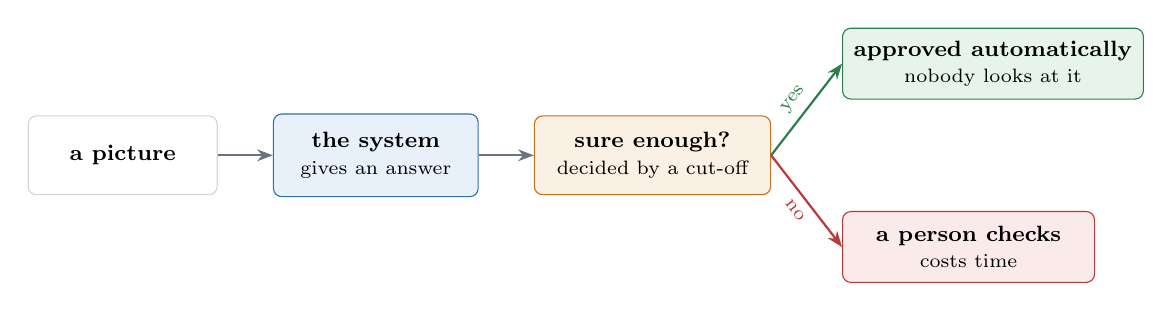
\begin{tikzpicture}[node distance=7mm]
\node[box,minimum width=2.4cm,minimum height=1.0cm] (p) {\textbf{a picture}};
\node[agentb,right=of p,minimum width=2.6cm] (s) {\textbf{the system}\\{\scriptsize gives an answer}};
\node[riskb,right=of s,minimum width=3.0cm,minimum height=1.0cm] (q) {\textbf{sure enough?}\\{\scriptsize decided by a cut-off}};
\node[okb,above right=2mm and 9mm of q,minimum width=3.2cm,minimum height=0.9cm] (ok) {\textbf{approved automatically}\\{\scriptsize nobody looks at it}};
\node[persb,below right=2mm and 9mm of q,minimum width=3.2cm,minimum height=0.9cm] (pe) {\textbf{a person checks}\\{\scriptsize costs time}};
\draw[arr] (p)--(s); \draw[arr] (s)--(q);
\draw[arr,okc] (q.east)--node[above,font=\scriptsize,sloped]{yes}(ok.west);
\draw[arr,pers] (q.east)--node[below,font=\scriptsize,sloped]{no}(pe.west);
\end{tikzpicture}
\vspace{8pt}
\begin{columns}[T,onlytextwidth]
\column{0.48\textwidth}
\begin{defbox}{The trade-off}
Approve \textbf{more} → less work, but more wrong labels slip through unseen.\\
Approve \textbf{less} → safer, but a person checks almost everything.
\end{defbox}
\column{0.48\textwidth}
\begin{defbox}{What the archive needs}
A rule that approves as much as possible \emph{and} a \textbf{promise}: ``at most 5 in 100 pictures are approved and wrong''.
\end{defbox}
\end{columns}
\note{This is the decision the whole thesis is about. Every answer is either approved automatically, and then nobody looks at it, or sent to a person. Approving more saves time but lets errors through. So the archive needs a rule plus a promise about how many errors get through.}
\end{frame}

\begin{frame}{The research question, and the hypothesis tested}
\renewcommand{\defboxfont}{\scriptsize}
\begin{columns}[T,onlytextwidth]
\column{0.49\textwidth}
\begin{defbox}{The research gap (Section 1.2)}
\begin{enumerate}\setlength\itemsep{1pt}
\item Detectors trained automatically for such archives are graded against their teachers, not against people.
\item No tested way to decide \textbf{how far} automatic answers on ambiguous historical pictures may be trusted.
\end{enumerate}
\end{defbox}
\begin{defbox}[colframe=risk,colbacktitle=riskbg,coltitle=risk]{The hypothesis}
Disagreement between models of different kinds signals \textbf{where} the system is wrong (from query-by-committee and deep ensembles).
\end{defbox}
\column{0.48\textwidth}
\footnotesize
\renewcommand{\arraystretch}{1.35}
\begin{tabularx}{\linewidth}{@{}>{\raggedright\arraybackslash}X >{\raggedright\arraybackslash}m{2.0cm}@{}}
\toprule
\textbf{Research question} & \textbf{Answer}\\
\midrule
RQ1 \;Disagreement as uncertainty? & \no{No}\\
RQ2 \;Less work, same error recall? & \yes{Yes}, with local calibration\\
RQ3 \;Contradictions add precision? & {\color{risk}\textbf{Partially}}\\
RQ4 \;Retrieval, cross-archive links? & {\color{risk}\textbf{Partially}}\\
\bottomrule
\end{tabularx}
\end{columns}
\takeaway{The system is the instrument; the result is the tested answer to the hypothesis.}
\note{The thesis is organised around a hypothesis, not around a pipeline. The gap is twofold: automatically trained detectors for these archives are graded against their teachers, not people, and there is no tested way to decide how far to trust them. The hypothesis is that disagreement between different models shows where the system is wrong; that is plausible from query-by-committee, deep ensembles and recent work on disagreement. I answer four research questions: RQ1 no, RQ2 yes with local calibration, RQ3 and RQ4 partially.}
\end{frame}

\begin{frame}{Related research (1 of 2): detection and disagreement}
\begin{tcbraster}[raster columns=3,raster equal height,raster column skip=8pt]
\relcard{Historical object detection}{Kim, Im \& Mandl 2024}
  {Transfer learning and pseudo-labels find objects in historical images without manual labels (F1 0.58 over 15 types).}
  {Grades such a student against \textbf{people}: 0.768 against its teacher, 0.146 against human boxes. The cause is the teacher; a better teacher reaches 0.210.}
\relcard{Committee and ensemble disagreement}{Seung et al.\ 1992; Lakshminarayanan et al.\ 2017}
  {Disagreement among models is used as a measure of uncertainty.}
  {Tests it with models of \textbf{different kinds}, in a test fixed in advance: never better than confidence, because 149 of 199 errors are shared.}
\relcard{Disagreement estimates error}{Jiang et al.\ 2022; Baek et al.\ 2022}
  {Disagreement estimates \emph{how many} answers are wrong, for models trained for the same task.}
  {Asks \emph{which picture} is wrong, with models of different kinds: the answer is negative here.}
\end{tcbraster}
\note{Where the thesis sits, part one. Kim, Im and Mandl showed that pseudo-labelling finds objects without manual labels; I grade such a student against people and trace its failure to the teacher. Committee and ensemble methods use disagreement as uncertainty; I test that with genuinely different models, in a test fixed in advance, and it does not beat confidence because most errors are shared. Jiang and Baek estimate how many answers are wrong; I ask which picture is wrong.}
\end{frame}

\begin{frame}{Related research (2 of 2): confidence, risk promises, illustrations}
\begin{tcbraster}[raster columns=3,raster equal height,raster column skip=8pt]
\relcard{Confidence and calibration}{Hendrycks \& Gimpel 2017; Guo et al.\ 2017; Ovadia et al.\ 2019}
  {A model's own confidence is a strong baseline for finding its errors; calibration degrades under shift.}
  {Confidence is the better router on historical prints, once each agent is mapped to a probability.}
\relcard{Conformal risk control}{Angelopoulos et al.\ 2024, 2025; Barber et al.\ 2023}
  {A risk promise without assumptions about the models, if new data are like the calibration data.}
  {Tests that condition on \textbf{random archive pictures}: 16.2\% approved and wrong with pool calibration, 5.4--5.9\% with archive calibration.}
\relcard{Multimodal models on book illustrations}{Piper \& Jiang 2026}
  {Strong models match people on concrete tasks and reproduce people's disagreement on others.}
  {The same limit: scene classes are recognised about as reliably as people agree ($\kappa = 0.34$).}
\end{tcbraster}
\note{Part two. A model's own confidence is a known strong baseline, and calibration degrades under shift; here confidence is the better router once each agent is mapped to a probability. Conformal risk control gives a promise if new data are like the calibration data; I test exactly that on random archive pictures. Piper and Jiang see the same limit as I do: models match people only as far as people agree.}
\end{frame}

% =====================================================================================================
\section{Words and measures}

\begin{frame}{Key words, in plain language}
\renewcommand{\defboxfont}{\scriptsize}
\begin{columns}[T,onlytextwidth]
\column{0.32\textwidth}
\begin{defbox}{Agent}
One model that looks at the picture and reports numbers. The corrected system has three.
\end{defbox}\vspace{3pt}
\begin{defbox}{Tier}
A layer of the system. Tier 1 decides; Tier 2 helpers only add notes; Tier 3 (paid models) was designed, not run.
\end{defbox}\vspace{3pt}
\begin{defbox}{Label (ground truth)}
The answer a person gave. Everything is measured against it.
\end{defbox}
\column{0.32\textwidth}
\begin{defbox}{Pseudo-label}
A label made by a model (the \emph{teacher}) instead of a person, used to train another model (the \emph{student}).
\end{defbox}\vspace{3pt}
\begin{defbox}{Zero-shot}
A model used without any training on this archive: we only give it sentences such as ``a family scene''.
\end{defbox}\vspace{3pt}
\begin{defbox}{Probability $p$}
A number from 0 to 1 that says how likely the answer is right, e.g.\ $p = 0.97$ for ``scene''.
\end{defbox}
\column{0.32\textwidth}
\begin{defbox}{Confidence and uncertainty $u$}
Confidence: how far $p$ is from a coin flip. Uncertainty is the opposite: $u = 1 - |p - 0.5|$.
\end{defbox}\vspace{3pt}
\begin{defbox}{Disagreement}
How much the agents' numbers differ for one picture. The first design used it as uncertainty.
\end{defbox}\vspace{3pt}
\begin{defbox}{Book-disjoint split}
Pictures of one book are only in training \emph{or} only in testing, never both.
\end{defbox}
\end{columns}
\note{A few words I will use throughout. An agent is one model. A pseudo-label is a label made by a model, not a person. Zero-shot means the model was never trained on this archive. Uncertainty is simply how close a probability is to a coin flip. Disagreement is how much the agents differ; that was the first design's idea of uncertainty.}
\end{frame}

\begin{frame}{The risk promise, in plain language}
\renewcommand{\defboxfont}{\scriptsize}
\begin{columns}[T,onlytextwidth]
\column{0.50\textwidth}
\begin{defbox}{Risk level $\alpha$ (alpha)}
The promise we ask for, e.g.\ $\alpha = 0.05$: at most 5 in 100 pictures may be \emph{approved and wrong}.
\end{defbox}\vspace{3pt}
\begin{defbox}{Cut-off $\lambda$ (lambda)}
Approve a picture if its uncertainty $u$ is below $\lambda$. A bigger $\lambda$ approves more.
\end{defbox}\vspace{3pt}
\begin{defbox}{Calibration set}
Labelled pictures kept apart, used only to choose $\lambda$.
\end{defbox}
\column{0.46\textwidth}
\centering

\begin{tikzpicture}[x=0.27cm,y=0.27cm]
\foreach \i in {0,...,9}{\foreach \j in {0,...,9}{
  \pgfmathtruncatemacro{\k}{\j*10+\i}
  \ifnum\k<5 \fill[pers] (\i,-\j) circle (0.38);
  \else\ifnum\k<76 \fill[okc!75] (\i,-\j) circle (0.38);
  \else \fill[line] (\i,-\j) circle (0.38);\fi\fi}}
\end{tikzpicture}\par\vspace{4pt}
\scriptsize
\tikz\fill[okc!75] circle (0.12); approved and right\quad
\tikz\fill[pers] circle (0.12); approved and wrong\quad
\tikz\fill[line] circle (0.12); sent to a person\par\vspace{4pt}
\footnotesize
\textbf{The promise counts the red dots among all 100}, not among the approved ones.\par\vspace{5pt}
\begin{defbox}{Conformal risk control (CRC)}
A method that picks the largest $\lambda$ for which the calibration pictures show the promise is kept, with a small safety margin.
\end{defbox}
\end{columns}
\note{The promise has three parts. Alpha is the promised risk. Lambda is the cut-off on uncertainty. The calibration set is a held-back set of labelled pictures used only to choose lambda. Conformal risk control picks the largest lambda that keeps the promise on those pictures. Important: the promise counts approved-and-wrong among all pictures, not the error rate among the approved ones.}
\end{frame}

\begin{frame}{The measures, explained with a picture}
\renewcommand{\defboxfont}{\scriptsize}
\begin{columns}[T,onlytextwidth]
\column{0.49\textwidth}
\begin{defbox}{AUROC: does a score rank errors first?}
Take one wrong and one right answer at random. AUROC = the chance the score gives the wrong one the higher value.\par
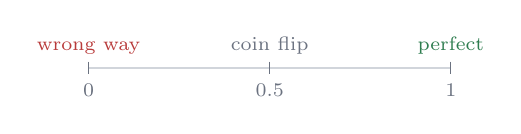
\begin{tikzpicture}[x=4.6cm,y=1cm]
\draw[line,thick] (0,0)--(1,0);
\foreach \x/\l in {0/0,0.5/0.5,1/1}{\draw[muted] (\x,0.08)--(\x,-0.08) node[below,font=\scriptsize]{\l};}
\node[font=\scriptsize,text=pers,above] at (0,0.05) {wrong way};
\node[font=\scriptsize,text=muted,above] at (0.5,0.05) {coin flip};
\node[font=\scriptsize,text=okc,above] at (1,0.05) {perfect};
\end{tikzpicture}
\end{defbox}\vspace{3pt}
\begin{defbox}{Balanced accuracy}
The share found per class, averaged over the classes, so a rare class counts as much as a common one.
\end{defbox}
\column{0.49\textwidth}
\begin{defbox}{AP50 (mAP50) for boxes}
A found box counts if it overlaps the person's box enough: \emph{IoU} (overlap ÷ union) $\geq 0.5$. AP50 summarises how many boxes are found and how many are right; mAP50 averages it over classes.\par\centering
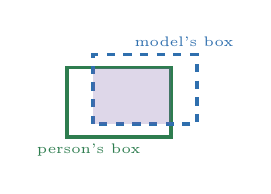
\begin{tikzpicture}[scale=0.55]
\draw[okc,very thick] (0,0) rectangle (2.4,1.6);
\draw[agent,very thick,dashed] (0.6,0.3) rectangle (3.0,1.9);
\fill[mapc,opacity=0.25] (0.6,0.3) rectangle (2.4,1.6);
\node[font=\tiny,text=okc] at (0.5,-0.3) {person's box};
\node[font=\tiny,text=agent] at (2.7,2.2) {model's box};
\end{tikzpicture}
\end{defbox}\vspace{3pt}
\begin{defbox}{Cohen's $\kappa$ (kappa)}
Agreement between two raters beyond chance: 0 = chance, 1 = always the same.
\end{defbox}
\end{columns}
\note{Four measures. AUROC asks whether a score puts the errors first: 0.5 is a coin flip, 1 is perfect, below 0.5 points the wrong way. Balanced accuracy averages over classes so rare classes count. AP50 is the standard detection measure: a box counts when it overlaps the human box by at least half. Kappa is agreement between people beyond chance.}
\end{frame}

\begin{frame}{Abbreviations used in this talk}
\small
\begin{columns}[T,onlytextwidth]
\column{0.49\textwidth}
\renewcommand{\arraystretch}{1.12}
\begin{tabular}{@{}>{\bfseries\color{navy}}l >{\raggedright\arraybackslash}p{5.3cm}@{}}
\toprule
AUROC & Area under the ROC curve: how well a score ranks errors first\\
AP50 & Average precision at box overlap (IoU) $\geq 0.5$\\
CRC & Conformal risk control (the risk promise)\\
IoU & Intersection over union: overlap of two boxes\\
$\kappa$ & Cohen's kappa: agreement between raters\\
$\alpha$, $\lambda$, $u$ & Risk level, cut-off, uncertainty\\
OCR & Optical character recognition (reading text)\\
\bottomrule
\end{tabular}
\column{0.49\textwidth}
\renewcommand{\arraystretch}{1.12}
\begin{tabular}{@{}>{\bfseries\color{navy}}l >{\raggedright\arraybackslash}p{5.3cm}@{}}
\toprule
VLM & Vision-language model: sees a picture, answers in words\\
YOLO & ``You only look once'': a fast object detector (YOLOv11)\\
SigLIP & An image--text matching model (zero-shot)\\
LLaVA & A vision-language model (LLaVA-OneVision 7B)\\
ESRGAN & The image restorer (Real-ESRGAN)\\
SAA & Scene-aware agreement: the first design's decision score\\
$U_{\text{SAA}}$ & The first design's disagreement score\\
\bottomrule
\end{tabular}
\end{columns}
\note{A reference slide; I will not read it out. The model names will each get their own slide next.}
\end{frame}

% =====================================================================================================
\section{The models}

\begin{frame}{Five models, one job each}
\footnotesize
\renewcommand{\arraystretch}{1.2}
\begin{tabularx}{\textwidth}{@{}>{\bfseries}l l X X r@{}}
\toprule
Role & Model & Takes in & Gives out & Time\\
\midrule
\rowcolor{soft}Restorer & Real-ESRGAN & the raw scan & a cleaner scan, twice the size & once\\
\color{agent}Object finder & YOLOv11m (retrained) & the picture & boxes with a class and a score $\to$ \textbf{8 numbers} & 0.06\,s\\
\color{agent}Scene matcher & SigLIP & the picture + 12 sentences & a score per sentence $\to$ \textbf{6 numbers} & \\
\color{agent}Describer & LLaVA-OneVision 7B & the picture + a yes/no question & how strongly it says ``yes'' $\to$ \textbf{13 numbers} & 1.56\,s\\
\rowcolor{soft}\color{tiertwo}Text reader & Kosmos-2.5 & the picture & the text it reads, as markdown (no positions) & 3.23\,s\\
\bottomrule
\end{tabularx}
\par\vspace{4pt}{\scriptsize\color{muted}Time per picture measured in the deployed run (object finder: the deployed detector) on one NVIDIA RTX A6000. The three blue agents decide; the text reader only feeds the Tier 2 helpers.}
\takeaway{Three different kinds of model, trained on different data: a detector, an image--text matcher and a vision-language model. Together they report \textbf{27 numbers} per picture.}
\note{Five models. The restorer cleans the scan once. Then three agents decide: the object finder, the scene matcher and the describer. They were chosen because they differ in architecture and training data, which is what a disagreement method needs. The text reader reads inscriptions but does not take part in the decision. Next, one slide per model: what goes in and what comes out.}
\end{frame}

\begin{frame}{Step \stepn{1} \,·\, The restorer (Real-ESRGAN)}
\begin{columns}[c,onlytextwidth]
\column{0.58\textwidth}
\centering
\begin{tikzpicture}
\node[inner sep=0] (in) {\includegraphics[height=3.8cm]{restorer_zoom_raw.jpg}};
\node[inner sep=0,right=10mm of in] (out) {\includegraphics[height=3.8cm]{restorer_zoom_restored.jpg}};
\draw[arr,line width=1.5pt] (in.east)--node[below=2pt,font=\scriptsize,text=muted]{ESRGAN}(out.west);
\node[io,above=1mm of in] {INPUT: raw scan};
\node[io,above=1mm of out] {OUTPUT: restored ($2\times$)};
\node[below=1mm of in.south east,xshift=5mm,font=\scriptsize,text=muted] {Running example, the woman's face, zoomed in: real pipeline files};
\end{tikzpicture}
\column{0.40\textwidth}
\small
\begin{itemize}\setlength\itemsep{4pt}
\item A neural network trained to turn a low-quality image into a sharp one (\emph{super-resolution}).
\item Run \textbf{once} per scan; every agent sees the restored picture.
\item The restored picture is never archival evidence: catalogue data always points to the original scan.
\end{itemize}
\begin{exbox}
Sharper, but the face is \textbf{redrawn}: she looks younger. Scene matcher: 0.329 restored vs 0.342 original. No gain; no result depends on it.
\end{exbox}
\end{columns}
\note{Step one. Real-ESRGAN restores the scan once, at twice the size, and all agents see the restored version. This is the woman's face from our running example, zoomed in, before and after, taken from the pipeline's own files. The lines get darker and the paper cleaner, but look at the woman's face: the nose and mouth are redrawn. The restorer invents detail. I tested whether it helps the scene matcher: it does not measurably, so no result depends on restoration.}
\end{frame}

\begin{frame}{Agent 1 \,·\, The object finder (YOLOv11m)}
\begin{columns}[T,onlytextwidth]
\column{0.30\textwidth}
\centering
\includegraphics[height=3.9cm]{object_finder_boxes.jpg}\par
{\scriptsize\color{muted}Its real boxes on the running example}
\column{0.33\textwidth}
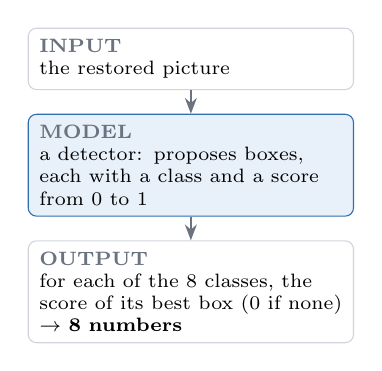
\begin{tikzpicture}[node distance=3mm,st/.style={box,text width=3.85cm,align=left,font=\scriptsize}]
\node[st] (i) {\textbf{\color{muted}INPUT}\\the restored picture};
\node[st,draw=agent,fill=agentbg,below=of i] (m) {\textbf{\color{muted}MODEL}\\a detector: proposes boxes, each with a class and a score from 0 to 1};
\node[st,below=of m] (o) {\textbf{\color{muted}OUTPUT}\\for each of the 8 classes, the score of its best box (0 if none) $\to$ \textbf{8 numbers}};
\draw[arr] (i)--(m); \draw[arr] (m)--(o);
\end{tikzpicture}
\column{0.34\textwidth}
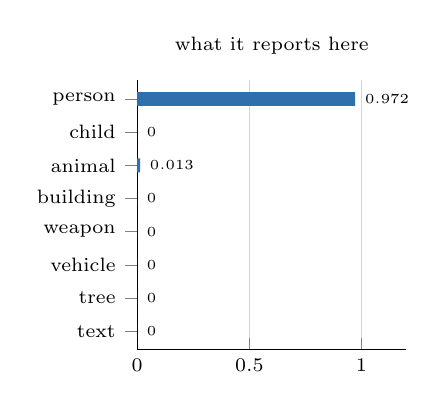
\begin{tikzpicture}
\begin{axis}[xbar,width=5.0cm,height=5.0cm,xmin=0,xmax=1.2,bar width=5pt,
  symbolic y coords={text,tree,vehicle,weapon,building,animal,child,person},ytick=data,
  nodes near coords,nodes near coords style={font=\tiny},axis lines*=left,xmajorgrids,grid style={line},
  enlarge y limits=0.08,title={\scriptsize what it reports here}]
\addplot[fill=agent,draw=none] coordinates {(0.972,person) (0,child) (0.013,animal) (0,building) (0,weapon) (0,vehicle) (0,tree) (0,text)};
\end{axis}
\end{tikzpicture}
\end{columns}
\takeaway{It boxes the boy (0.97) and the woman (0.90) as \emph{person}, never as \emph{child}; the hen gets only 0.01. Retrained on boxes from a stronger \emph{teacher} (Grounding DINO) on 11,028 archive pictures.}
\note{The object finder is a YOLOv11 detector. It proposes boxes with a class and a score; for each class we keep the score of its best box, so 8 numbers. In our running example you see its real boxes: the boy as a person at 0.97, the woman as a person at 0.90, but neither as a child, and the hen under the bench only at 0.01. So the child score is 0 and the animal score 0.01. It was retrained on boxes from a stronger teacher model.}
\end{frame}

\begin{frame}{Agent 2 \,·\, The scene matcher (SigLIP)}
\begin{columns}[T,onlytextwidth]
\column{0.56\textwidth}
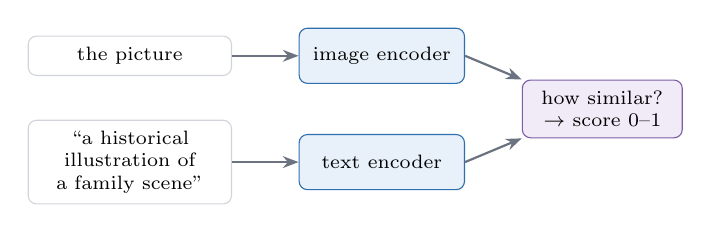
\begin{tikzpicture}[e/.style={box,draw=agent,fill=agentbg,minimum width=2.1cm,minimum height=0.7cm,font=\scriptsize}]
\node[box,text width=2.3cm,font=\scriptsize] (img) at (0,0) {the picture};
\node[box,text width=2.3cm,font=\scriptsize] (txt) at (0,-1.35) {``a historical illustration of a family scene''};
\node[e] (ei) at (3.2,0) {image encoder};
\node[e] (et) at (3.2,-1.35) {text encoder};
\node[mapb,text width=1.75cm,font=\scriptsize] (sim) at (6.0,-0.675) {how similar?\\$\to$ score 0--1};
\draw[arr] (img)--(ei); \draw[arr] (txt)--(et);
\draw[arr] (ei.east)--(sim.north west); \draw[arr] (et.east)--(sim.south west);
\end{tikzpicture}\par\vspace{6pt}
\begin{defbox}{Input and output}
\textbf{Input:} the picture + 12 sentences: 5 scene sentences and 7 ``not a scene'' sentences (printed text, sheet music, ornament, blank page, title page, table of numbers, map).\\[2pt]
\textbf{Output:} 5 scene scores + the highest ``not a scene'' score = \textbf{6 numbers}. Each sentence is scored on its own, so it can say ``none fits''.
\end{defbox}
\column{0.41\textwidth}
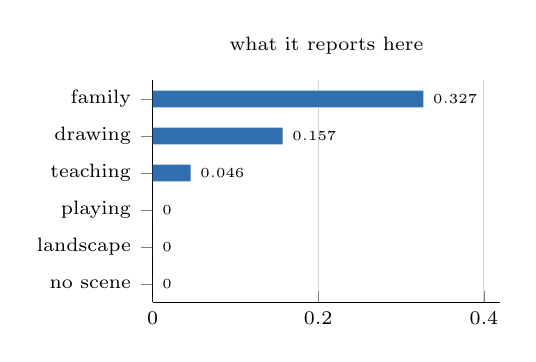
\begin{tikzpicture}
\begin{axis}[xbar,width=6.0cm,height=4.4cm,xmin=0,xmax=0.42,bar width=6pt,
  symbolic y coords={no scene,landscape,playing,teaching,drawing,family},ytick=data,
  nodes near coords,nodes near coords style={font=\tiny},axis lines*=left,xmajorgrids,grid style={line},
  title={\scriptsize what it reports here},enlarge y limits=0.1,xtick={0,0.2,0.4}]
\addplot[fill=agent,draw=none] coordinates {(0.327,family) (0.157,drawing) (0.046,teaching) (0,playing) (0,landscape) (0,no scene)};
\end{axis}
\end{tikzpicture}\par
\footnotesize\emph{Zero-shot}: SigLIP was never trained on this archive; it only compares the picture with sentences.
\end{columns}
\note{SigLIP turns the picture and a sentence into vectors and measures how similar they are. We give it five scene sentences and seven not-a-scene sentences. Each is scored on its own, so the model can say that none fits; the old design used a forced choice that could not say no scene. For our example, family scores highest.}
\end{frame}

\begin{frame}{Agent 3 \,·\, The describer (LLaVA-OneVision 7B)}
\begin{columns}[T,onlytextwidth]
\column{0.50\textwidth}
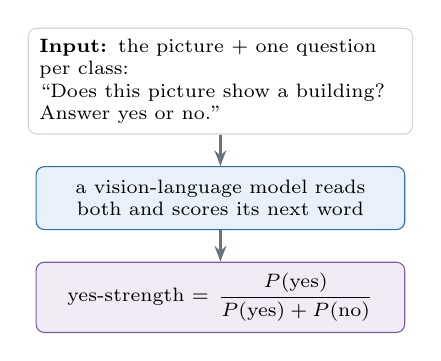
\begin{tikzpicture}[node distance=4mm]
\node[box,text width=4.6cm,align=left,font=\scriptsize] (q) {\textbf{Input:} the picture + one question per class:\\``Does this picture show a building? Answer yes or no.''};
\node[agentb,below=of q,text width=4.4cm,minimum height=0.8cm,font=\scriptsize] (m) {a vision-language model reads both and scores its next word};
\node[mapb,below=of m,text width=4.4cm,font=\scriptsize] (o) {yes-strength $= \dfrac{P(\text{yes})}{P(\text{yes}) + P(\text{no})}$};
\draw[arr] (q)--(m); \draw[arr] (m)--(o);
\end{tikzpicture}\par\vspace{4pt}
\footnotesize 8 object questions + 5 scene questions = \textbf{13 numbers}. We read the model's probabilities, not its text, so we get a number between 0 and 1.
\column{0.48\textwidth}
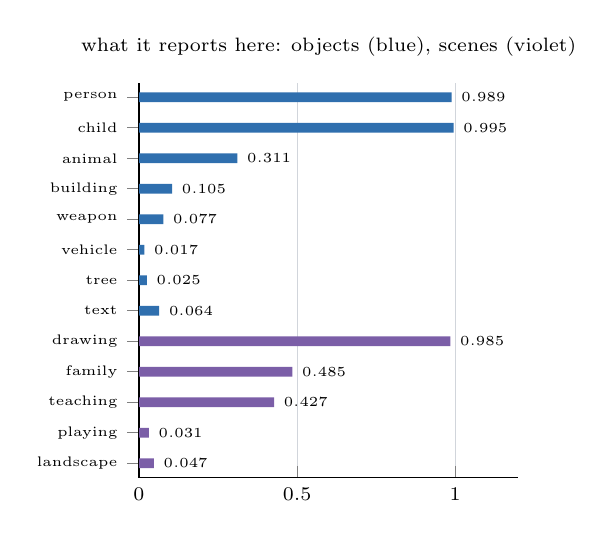
\begin{tikzpicture}
\begin{axis}[xbar,width=6.4cm,height=6.6cm,xmin=0,xmax=1.2,bar width=3.5pt,
  symbolic y coords={landscape,playing,teaching,family,drawing,text,tree,vehicle,weapon,building,animal,child,person},
  ytick={landscape,playing,teaching,family,drawing,text,tree,vehicle,weapon,building,animal,child,person},bar shift=0pt,
  y tick label style={font=\tiny},
  nodes near coords,nodes near coords style={font=\tiny},axis lines*=left,xmajorgrids,grid style={line},
  title={\scriptsize what it reports here: objects (blue), scenes (violet)},enlarge y limits=0.04,xtick={0,0.5,1}]
\addplot[fill=agent,draw=none] coordinates {(0.989,person) (0.995,child) (0.311,animal) (0.105,building) (0.077,weapon) (0.017,vehicle) (0.025,tree) (0.064,text)};
\addplot[fill=mapc,draw=none] coordinates {(0.985,drawing) (0.485,family) (0.427,teaching) (0.031,playing) (0.047,landscape)};
\end{axis}
\end{tikzpicture}
\end{columns}
\note{The describer is LLaVA-OneVision, a 7-billion-parameter vision-language model. We ask one yes-or-no question per class and read the probability of yes against no from the model, not its written answer. That gives 13 numbers. Here it sees the boy, child 0.995, which the object finder missed, and it leans towards drawing among the scenes.}
\end{frame}

\begin{frame}{The text reader (Kosmos-2.5) and the 27 numbers}
\begin{columns}[T,onlytextwidth]
\column{0.47\textwidth}
\begin{defbox}{Text reader: Kosmos-2.5}
\begin{minipage}[t]{0.40\linewidth}\vspace{0pt}
\includegraphics[width=\linewidth]{text_reader_frog.jpg}\par
{\tiny\color{muted}Printed: Der Frosch / Rana / la r\'ana / la grenouille / the frog\par}
\end{minipage}\hfill
\begin{minipage}[t]{0.56\linewidth}\vspace{0pt}
{\scriptsize\color{muted}What it returned:}\\[1pt]
{\ttfamily\scriptsize Der \textcolor{red!70!black}{Srofch}.\\ Name: La rana.\\ I am a\\ rana.\\ I am a\\ rana.\\ \dots}\\[1pt]
{\scriptsize ``I am a / rana.'' \textbf{32 times}}
\end{minipage}\\[4pt]
\footnotesize\textbf{Not used to decide.} About half its outputs loop like this; of its ``real text'', only 52.5\% comes from pictures that have text. It feeds the Tier 2 inscription reader only.
\end{defbox}
\column{0.50\textwidth}
\centering
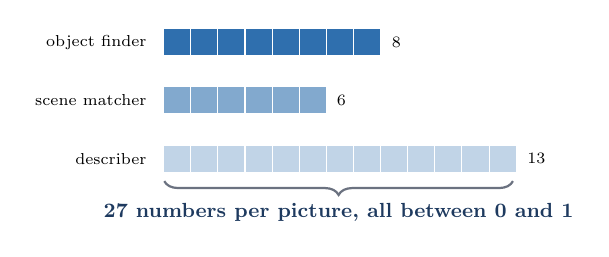
\begin{tikzpicture}[scale=0.82,transform shape,n/.style={draw=white,fill=agent,minimum size=4.2mm,inner sep=0},
                    s/.style={draw=white,fill=agent!60,minimum size=4.2mm,inner sep=0},
                    d/.style={draw=white,fill=agent!30,minimum size=4.2mm,inner sep=0}]
\foreach \i in {0,...,7} \node[n] at (\i*0.42,0) {};
\foreach \i in {0,...,5} \node[s] at (\i*0.42,-0.9) {};
\foreach \i in {0,...,12} \node[d] at (\i*0.42,-1.8) {};
\node[anchor=east,font=\scriptsize] at (-0.35,0) {object finder};
\node[anchor=east,font=\scriptsize] at (-0.35,-0.9) {scene matcher};
\node[anchor=east,font=\scriptsize] at (-0.35,-1.8) {describer};
\node[font=\scriptsize,anchor=west] at (3.2,0) {8};
\node[font=\scriptsize,anchor=west] at (2.35,-0.9) {6};
\node[font=\scriptsize,anchor=west] at (5.3,-1.8) {13};
\draw[decorate,decoration={brace,amplitude=5pt,mirror},thick,muted] (-0.2,-2.15)--(5.2,-2.15) node[midway,below=6pt,font=\small\bfseries,text=navy]{27 numbers per picture, all between 0 and 1};
\end{tikzpicture}\par\vspace{8pt}
\footnotesize The three agents \textbf{never see each other's numbers}. What happens to the 27 numbers depends on the design: first the old one, then the corrected one.
\end{columns}
\note{The text reader reads the text printed on a picture. Here is its real output for the frog page: it reads Der Srofch instead of Der Frosch, invents a line, misses the French and English names, and then repeats I am a, rana, thirty-two times. That is why it does not decide anything: about half of its outputs loop, and its real-text bucket is only about half right. So the decision rests on 27 numbers from three independent agents.}
\end{frame}

% =====================================================================================================
\section{The first design}

\begin{frame}{The first design, as deployed on all 12,110 pictures}
\centering
\resizebox{\linewidth}{!}{%
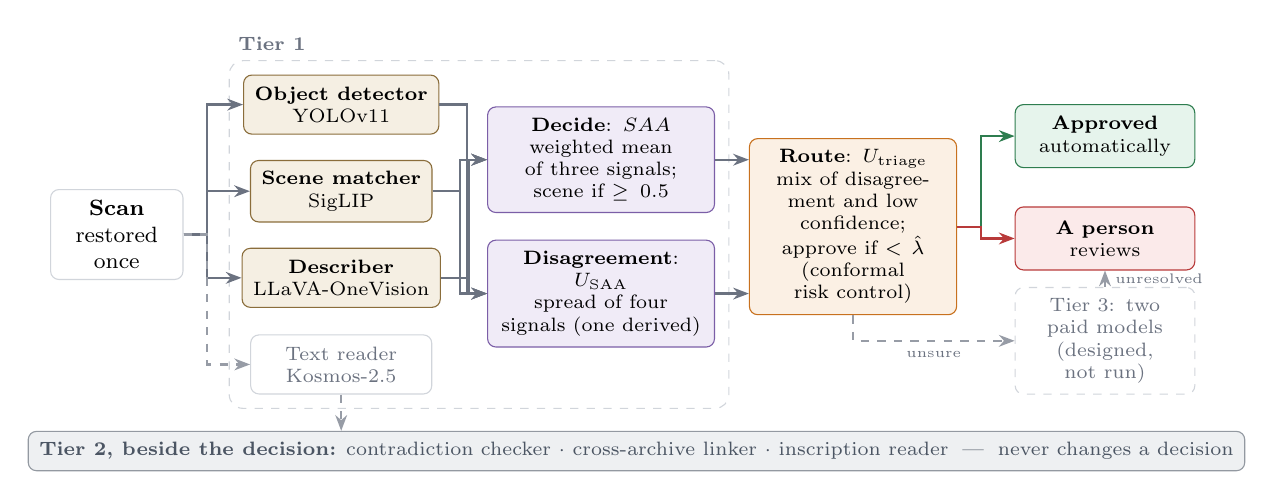
\begin{tikzpicture}[font=\scriptsize,
  m/.style={box,draw=oldc,fill=oldbg,minimum width=2.3cm,minimum height=0.75cm,font=\scriptsize},
  c/.style={box,draw=mapc,fill=mapbg,text width=2.6cm,minimum height=1.25cm,font=\scriptsize},
  lab/.style={font=\scriptsize\bfseries,text=muted}]
\node[box,text width=1.4cm,minimum height=1.1cm] (scan) at (0,0) {\textbf{Scan}\\restored once};
\node[m] (det) at (2.85,1.65) {\textbf{Object detector}\\YOLOv11};
\node[m] (sig) at (2.85,0.55) {\textbf{Scene matcher}\\SigLIP};
\node[m] (vlm) at (2.85,-0.55) {\textbf{Describer}\\LLaVA-OneVision};
\node[m,draw=line,fill=white,text=muted] (ocr) at (2.85,-1.65) {Text reader\\Kosmos-2.5};
\foreach \a in {det,sig,vlm} \draw[arr] (scan.east) -- ++(0.3,0) |- (\a.west);
\draw[dashedarr] (scan.east) -- ++(0.3,0) |- (ocr.west);
\node[c] (saa) at (6.15,0.95) {\textbf{Decide}: $SAA$\\weighted mean of three signals; scene if $\ge 0.5$};
\node[c] (usaa) at (6.15,-0.75) {\textbf{Disagreement}: $U_{\text{SAA}}$\\spread of four signals (one derived)};
\foreach \a in {det,sig,vlm}{\draw[arr] (\a.east) -- ++(0.35,0) |- (saa.west); \draw[arr] (\a.east) -- ++(0.35,0) |- (usaa.west);}
\node[riskb,text width=2.35cm,minimum height=1.6cm,font=\scriptsize] (route) at (9.35,0.1) {\textbf{Route}: $U_{\text{triage}}$\\mix of disagreement and low confidence; approve if $< \hat\lambda$\\(conformal risk control)};
\draw[arr] (saa.east) -- (route.west |- saa.east);
\draw[arr] (usaa.east) -- (route.west |- usaa.east);
\node[okb,text width=2.0cm,minimum height=0.8cm,font=\scriptsize] (ok) at (12.55,1.25) {\textbf{Approved}\\automatically};
\node[persb,text width=2.0cm,minimum height=0.8cm,font=\scriptsize] (pe) at (12.55,-0.05) {\textbf{A person}\\reviews};
\node[box,draw=line,dashed,text=muted,text width=2.0cm,font=\scriptsize] (t3) at (12.55,-1.35) {Tier 3: two paid models (designed, not run)};
\draw[arr,okc] (route.east) -- ++(0.3,0) |- (ok.west);
\draw[arr,pers] (route.east) -- ++(0.3,0) |- (pe.west);
\draw[dashedarr] (route.south) |- node[pos=0.75,below,font=\tiny,text=muted]{unsure} (t3.west);
\draw[dashedarr] (t3.north) -- node[right,font=\tiny,text=muted]{unresolved} (pe.south);
\node[greyb,minimum width=14.4cm,font=\scriptsize] (t2) at (6.6,-2.75) {\textbf{Tier 2, beside the decision:} contradiction checker $\cdot$ cross-archive linker $\cdot$ inscription reader \;---\; never changes a decision};
\draw[dashedarr] (ocr.south) -- (ocr.south |- t2.north);
\begin{scope}[on background layer]
\node[draw=line,dashed,rounded corners=5pt,inner sep=5pt,fit=(det)(ocr)(saa)(usaa),label={[lab,anchor=south west]north west:Tier 1}] {};
\end{scope}
\end{tikzpicture}}
\par\vspace{4pt}{\footnotesize\color{muted}Figure 2.1 of the thesis, drawn left to right. The key idea: \textbf{disagreement means doubt}.}
\note{This is the system as first built and run over the whole archive, Figure 2.1 of the thesis. Four models; their outputs become signals. Two formulas: SAA decides scene or not, U-SAA measures disagreement. The routing score mixes disagreement with low confidence, and conformal risk control sets the cut-off. The key idea: disagreement means doubt.}
\end{frame}

\begin{frame}{How the first design turned answers into four numbers}
\small
\renewcommand{\arraystretch}{1.2}
\begin{tabularx}{\textwidth}{@{}>{\bfseries\color{oldc}}l X X l@{}}
\toprule
Signal & Taken from & Rule & Possible values\\
\midrule
$A^{\text{object}}$ & how many objects the describer listed & count $\div$ 3, at most 1 & 0, $\tfrac13$, $\tfrac23$, 1\\
$A^{\text{scene}}$ & the describer's scene confidence & as stored & in practice 0.5 or 1\\
$A^{\text{vlm}}$ & did the describer list any object? & yes $\to$ 1, no $\to$ 0 & 0 or 1\\
$A^{\text{agree}}$ & computed from two of the above & $1 - |A^{\text{object}} - A^{\text{vlm}}|$ & fixed by them\\
\bottomrule
\end{tabularx}
\vspace{6pt}
\begin{columns}[T,onlytextwidth]
\column{0.50\textwidth}
\begin{exbox}
``a man and a horse'' $\to$ 2 objects:\\
$A^{\text{object}} = \tfrac23$, $A^{\text{vlm}} = 1$, $A^{\text{agree}} = 1 - |\tfrac23 - 1| = \tfrac23$.
\end{exbox}
\column{0.46\textwidth}
\begin{keybox}[colback=persbg,colframe=pers]
Despite their names, all four came from \textbf{one model's answer}: two measurements, not four.
\end{keybox}
\end{columns}
\note{This is how the deployed run actually computed its four signals, which the audit in the thesis found. The object signal was the describer's object count divided by three, not the detector. The scene signal was the describer's own scene confidence. So all four numbers came from one model's answer.}
\end{frame}

\begin{frame}{From four numbers to ``approve or check''}
\begin{columns}[T,onlytextwidth]
\column{0.52\textwidth}
\begin{defbox}{Decide}
$SAA = 0.6\,A^{\text{object}} + 0.2\,A^{\text{scene}} + 0.2\,A^{\text{vlm}}$\quad scene if $SAA \geq 0.5$
\end{defbox}\vspace{3pt}
\begin{defbox}{Measure disagreement}
$U_{\text{SAA}}$ = standard deviation of the four signals
\end{defbox}\vspace{3pt}
\begin{defbox}{Route}
$U_{\text{triage}} = 0.6\,U_{\text{SAA}} + 0.4\,(1 - \text{mean of the four})$\\
approve if $U_{\text{triage}} < \hat\lambda = 0.372$ (at a 5\% promise)
\end{defbox}
\column{0.45\textwidth}
\begin{exbox}
$A^{\text{object}} = \tfrac23$, $A^{\text{scene}} = 1$, $A^{\text{vlm}} = 1$, $A^{\text{agree}} = \tfrac23$\\[3pt]
$SAA = 0.6\cdot\tfrac23 + 0.2 + 0.2 = \mathbf{0.80}$ $\to$ scene\\[3pt]
spread $= 0.19$, mean $= 0.83$\\
$U_{\text{triage}} = 0.6\cdot0.19 + 0.4\cdot0.17 = \mathbf{0.18}$\\[3pt]
$0.18 < 0.372$ $\to$ \yes{approved}
\end{exbox}
\vspace{3pt}
{\footnotesize\color{muted}All weights were set by hand. Learning them later changed nothing that matters.}
\end{columns}
\note{Three formulas. SAA decides, with weights 0.6, 0.2, 0.2. U-SAA is the spread of the four signals: the disagreement. The routing score mixes disagreement with low confidence, and a picture is approved below the cut-off 0.372 found by conformal risk control. For the example the picture is a scene and is approved.}
\end{frame}

\begin{frame}{Problem 1 \,·\, The whole archive fell into eight states}
\begin{columns}[c,onlytextwidth]
\column{0.58\textwidth}
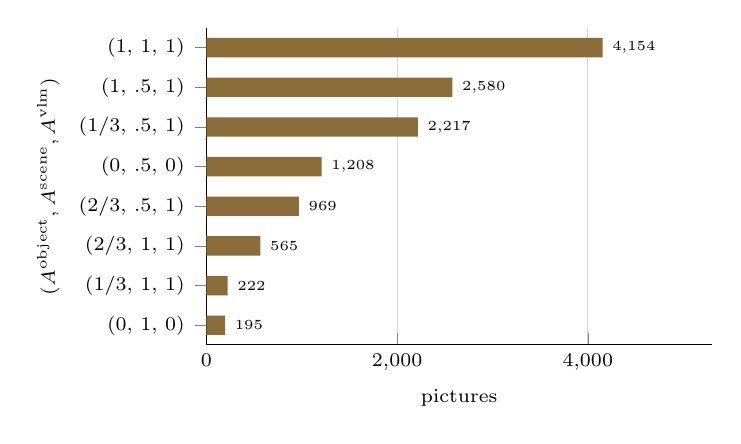
\begin{tikzpicture}
\begin{axis}[xbar,width=8.0cm,height=5.6cm,every node near coord/.append style={anchor=west},xmin=0,xmax=5300,bar width=7pt,xtick={0,2000,4000},xticklabels={0,{2,000},{4,000}},
  ytick={1,...,8},yticklabels={{(0, 1, 0)},{(1/3, 1, 1)},{(2/3, 1, 1)},{(2/3, .5, 1)},{(0, .5, 0)},{(1/3, .5, 1)},{(1, .5, 1)},{(1, 1, 1)}},y tick label style={font=\scriptsize},x tick label style={font=\scriptsize},
  xlabel={\scriptsize pictures},ylabel={\scriptsize $(A^{\text{object}}, A^{\text{scene}}, A^{\text{vlm}})$},
  nodes near coords,nodes near coords style={font=\tiny},axis lines*=left,xmajorgrids,grid style={line},
  scaled x ticks=false,enlarge y limits=0.07]
\addplot[fill=oldc,draw=none,point meta=explicit symbolic] coordinates {(4154,8) [4,154] (2580,7) [2,580] (2217,6) [2,217] (1208,5) [1,208] (969,4) [969] (565,3) [565] (222,2) [222] (195,1) [195]};
\end{axis}
\end{tikzpicture}
\column{0.40\textwidth}
\begin{defbox}{Why exactly eight}
$A^{\text{object}}$ has 4 values $\times$ $A^{\text{scene}}$ has 2 values $= 8$. $A^{\text{vlm}}$ adds nothing: it is 1 whenever $A^{\text{object}} > 0$.
\end{defbox}\vspace{4pt}
\begin{keybox}[colback=persbg,colframe=pers]
Every picture in a row gets the \textbf{same decision} and the \textbf{same uncertainty}. 4,154 + 2,580 + … + 195 = 12,110.
\end{keybox}
\end{columns}
\note{Because the signals came from one count and one stored confidence, the whole archive fits in eight rows. Every picture in a row gets the same decision and the same uncertainty. A ranking of errors with only eight values cannot be fine-grained.}
\end{frame}

\begin{frame}{Problem 2 \,·\, A model graded by its own teacher looks good}
\begin{columns}[c,onlytextwidth]
\column{0.55\textwidth}
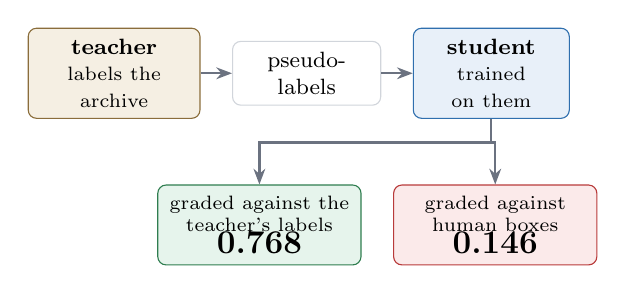
\begin{tikzpicture}[node distance=4mm]
\node[oldb,text width=1.9cm] (t) {\textbf{teacher}\\{\scriptsize labels the archive}};
\node[box,right=of t,text width=1.6cm] (pl) {pseudo-labels};
\node[agentb,right=of pl,minimum width=1.9cm,text width=1.7cm] (s) {\textbf{student}\\{\scriptsize trained on them}};
\draw[arr] (t)--(pl); \draw[arr] (pl)--(s);
\node[okb,below=10mm of pl,xshift=-6mm,text width=2.3cm,font=\scriptsize] (g1) {graded against the teacher's labels\\{\large\textbf{0.768}}};
\node[persb,right=4mm of g1,text width=2.3cm,font=\scriptsize] (g2) {graded against human boxes\\{\large\textbf{0.146}}};
\draw[arr] (s.south) -- ++(0,-3mm) -| (g1.north);
\draw[arr] (s.south) -- ++(0,-3mm) -| (g2.north);
\end{tikzpicture}
\par\vspace{4pt}\footnotesize mAP50, same model, same validator, two kinds of ground truth (300 hand-boxed pictures).
\column{0.42\textwidth}
\small
\begin{itemize}\setlength\itemsep{4pt}
\item The teacher never labelled child, building, weapon, vehicle or text; 88\% of its boxes were persons.
\item Of 128 objects the student misses, \textbf{126} were never in the teacher's labels.
\item With the thesis's own evaluator: 0.123; a better teacher (Grounding DINO) lifts it to \yes{0.210}.
\end{itemize}
\end{columns}
\takeaway{Nothing inside the pipeline noticed the collapse. That is why the system needs an outside check, and why the thesis measures against people.}
\note{The second problem: the deployed detector was a student trained on a teacher's pseudo-labels. Graded against those labels it scores 0.768; graded against people, 0.146. The teacher simply never labelled most classes. With a better teacher the student improves from 0.123 to 0.210 on the thesis's own evaluator.}
\end{frame}

\begin{frame}{Problem 3 \,·\, Disagreement does not find the errors}
\begin{columns}[T,onlytextwidth]
\column{0.56\textwidth}
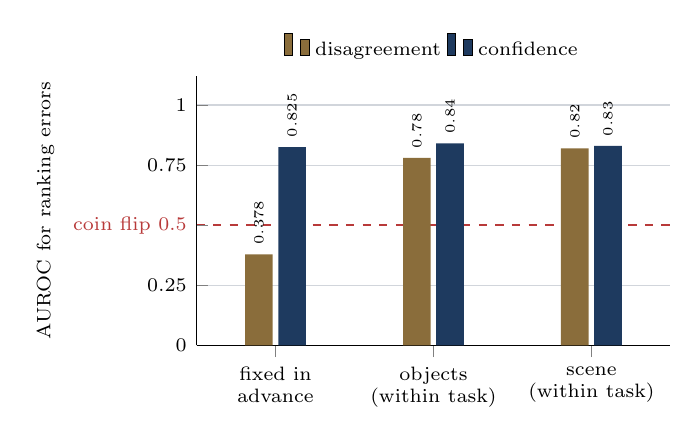
\begin{tikzpicture}
\begin{axis}[ybar,width=7.6cm,height=5.0cm,ymin=0,ymax=1,bar width=10pt,
  symbolic x coords={pre-registered test,objects,scene presence},xtick=data,xticklabels={{fixed in\\advance},{objects\\(within task)},{scene\\(within task)}},
  x tick label style={font=\scriptsize,align=center},y tick label style={font=\scriptsize},ylabel={\scriptsize AUROC for ranking errors},
  nodes near coords,nodes near coords style={font=\tiny,/pgf/number format/precision=3,rotate=90,anchor=west},axis lines*=left,ymajorgrids,grid style={line},
  legend style={font=\scriptsize,at={(0.5,1.02)},anchor=south,legend columns=2,draw=none},enlarge x limits=0.25,ymax=1.12,ytick={0,0.25,0.75,1},
  extra y ticks={0.5},extra y tick labels={\color{pers}coin flip 0.5},extra y tick style={grid=major,grid style={pers,dashed,thick},tick label style={font=\tiny}}]
\addplot[fill=oldc,draw=none] coordinates {(pre-registered test,0.378) (objects,0.78) (scene presence,0.82)};
\addplot[fill=navy,draw=none] coordinates {(pre-registered test,0.825) (objects,0.84) (scene presence,0.83)};
\legend{disagreement,confidence}
\end{axis}
\end{tikzpicture}
\par\footnotesize\color{muted}Pre-registered: fixed in writing before it was run (300 hand-labelled pictures). It asked object disagreement about scene errors; within each task disagreement is informative, but never above confidence.
\column{0.41\textwidth}
\centering
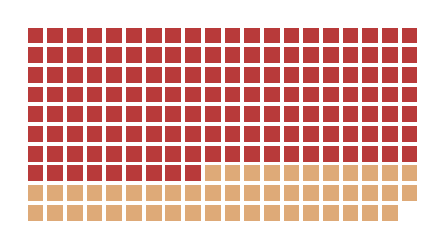
\begin{tikzpicture}[x=0.25cm,y=0.25cm]
\foreach \k in {0,...,198}{
  \pgfmathtruncatemacro{\i}{mod(\k,20)}\pgfmathtruncatemacro{\j}{\k/20}
  \ifnum\k<149 \fill[pers] (\i,-\j) rectangle ++(0.8,0.8);
  \else \fill[risk!60] (\i,-\j) rectangle ++(0.8,0.8);\fi}
\end{tikzpicture}\par\vspace{3pt}
\footnotesize
\tikz\fill[pers] (0,0) rectangle (0.2,0.2); all three agents wrong together: \textbf{149}\\
\tikz\fill[risk!60] (0,0) rectangle (0.2,0.2); some agents right: 50\quad(of 199 errors)\par\vspace{4pt}
\begin{keybox}[colback=persbg,colframe=pers]
When all agents make the same mistake, they \emph{agree}, so disagreement cannot see it.
\end{keybox}
\end{columns}
\note{The central test, fixed before it was run. Disagreement ranks the errors at 0.378, confidence at 0.825. Careful: that test used object disagreement for scene errors. Measured within each task, disagreement reaches 0.78 and 0.82, but confidence is still at least as good. The reason is on the right: on 149 of 199 errors all three agents are wrong together, so they agree.}
\end{frame}

\begin{frame}{From diagnosis to design}
\footnotesize
\renewcommand{\arraystretch}{1.15}
\begin{tabularx}{\textwidth}{@{}>{\raggedright\arraybackslash\color{oldc}}X c >{\raggedright\arraybackslash\color{navy}}X@{}}
\toprule
\textbf{What went wrong in the first design} & & \textbf{What the corrected design does}\\
\midrule
Four signals read from one model's answer & $\to$ & each agent reports what it \textbf{measures} (27 numbers)\\
Agreement term computed from two other signals & $\to$ & \textbf{removed}\\
Scene matcher had to pick a scene; could not say ``none'' & $\to$ & a separate \textbf{``no scene''} score\\
Signals on different scales, mixed with hand-set weights & $\to$ & each agent \textbf{mapped to a probability}, learned from labels\\
Routing by disagreement & $\to$ & routing by \textbf{confidence}\\
Conformal risk control & $\to$ & \textbf{unchanged}\\
\bottomrule
\end{tabularx}
\takeaway{Keep what worked (the risk promise), replace what the evidence rejected (disagreement as uncertainty).}
\note{Each problem leads to one change. Real measurements instead of one count; no derived agreement term; a no-scene score; a common probability scale learned from labels; and routing by confidence. The risk promise is kept.}
\end{frame}

% =====================================================================================================
\section{The corrected design}

\begin{frame}{The corrected design at a glance}
\centering
\resizebox{\linewidth}{!}{%
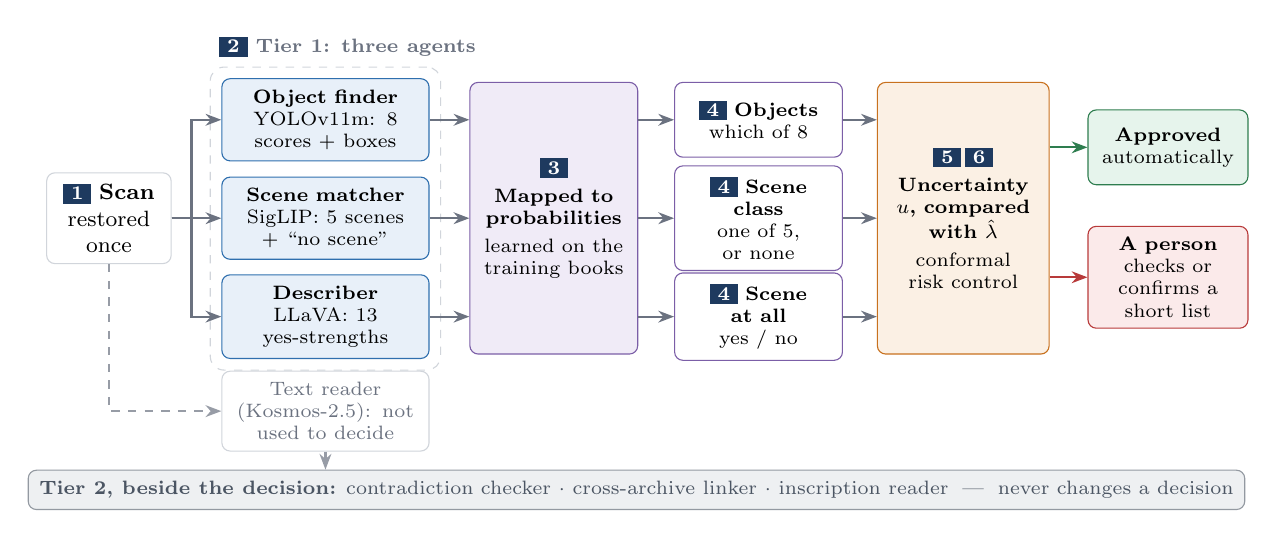
\begin{tikzpicture}[font=\scriptsize,
  a/.style={box,draw=agent,fill=agentbg,text width=2.35cm,minimum height=0.95cm,font=\scriptsize},
  o/.style={box,draw=mapc,fill=white,text width=1.85cm,minimum height=0.95cm,font=\scriptsize},
  lab/.style={font=\scriptsize\bfseries,text=muted}]
\node[box,text width=1.3cm,minimum height=1.1cm] (scan) at (0,0) {\stepn{1} \textbf{Scan}\\restored once};
\node[a] (det) at (2.75,1.25) {\textbf{Object finder}\\YOLOv11m: 8 scores + boxes};
\node[a] (sig) at (2.75,0) {\textbf{Scene matcher}\\SigLIP: 5 scenes + ``no scene''};
\node[a] (vlm) at (2.75,-1.25) {\textbf{Describer}\\LLaVA: 13 yes-strengths};
\foreach \a in {det,sig,vlm} \draw[arr] (scan.east) -- ++(0.25,0) |- (\a.west);
\node[mapb,text width=1.85cm,minimum height=3.45cm,font=\scriptsize] (map) at (5.65,0) {\stepn{3}\\[2pt]\textbf{Mapped to probabilities}\\[2pt]learned on the training books};
\foreach \a in {det,sig,vlm} \draw[arr] (\a.east) -- (map.west |- \a.east);
\node[o] (ob) at (8.25,1.25) {\stepn{4} \textbf{Objects}\\which of 8};
\node[o] (sc) at (8.25,0) {\stepn{4} \textbf{Scene class}\\one of 5, or none};
\node[o] (sa) at (8.25,-1.25) {\stepn{4} \textbf{Scene at all}\\yes / no};
\foreach \o in {ob,sc,sa} \draw[arr] (map.east |- \o.west) -- (\o.west);
\node[riskb,text width=1.9cm,minimum height=3.45cm,font=\scriptsize] (crc) at (10.85,0) {\stepn{5}\,\stepn{6}\\[2pt]\textbf{Uncertainty $u$, compared with $\hat\lambda$}\\[2pt]conformal risk control};
\foreach \o in {ob,sc,sa} \draw[arr] (\o.east) -- (crc.west |- \o.east);
\node[okb,text width=1.75cm,minimum height=0.95cm,font=\scriptsize] (ok) at (13.45,0.9) {\textbf{Approved}\\automatically};
\node[persb,text width=1.75cm,minimum height=0.95cm,font=\scriptsize] (pe) at (13.45,-0.75) {\textbf{A person}\\checks or confirms a short list};
\draw[arr,okc] (crc.east |- ok.west) -- (ok.west);
\draw[arr,pers] (crc.east |- pe.west) -- (pe.west);
\node[box,draw=line,text=muted,text width=2.35cm,font=\scriptsize] (ocr) at (2.75,-2.45) {Text reader (Kosmos-2.5): not used to decide};
\draw[dashedarr] (scan.south) |- (ocr.west);
\node[greyb,minimum width=14.4cm,font=\scriptsize] (t2) at (6.7,-3.45) {\textbf{Tier 2, beside the decision:} contradiction checker $\cdot$ cross-archive linker $\cdot$ inscription reader \;---\; never changes a decision};
\draw[dashedarr] (ocr.south) -- (ocr.south |- t2.north);
\begin{scope}[on background layer]
\node[draw=line,dashed,rounded corners=5pt,inner sep=4pt,fit=(det)(vlm),label={[lab,anchor=south west]north west:{\stepn{2} Tier 1: three agents}}] {};
\end{scope}
\end{tikzpicture}}
\par\vspace{3pt}{\footnotesize\color{muted}Figure 6.1 of the thesis, left to right. No Agreement term; \textbf{confidence} decides what a person checks.}
\note{The corrected design, Figure 6.1 of the thesis. Same scan, three agents reporting what they measure, each report mapped to probabilities, three answers each with an uncertainty, and conformal risk control deciding what is approved, what goes to a person, and what becomes a short list. The next slides take the six steps one at a time with our running example.}
\end{frame}

\begin{frame}{Learned once, then the same steps for every picture}
\begin{columns}[T,onlytextwidth]
\column{0.48\textwidth}
\textbf{\color{navy}ONCE, before use}\quad{\footnotesize\color{muted}1,250 labelled pictures, split by book}\par\vspace{6pt}
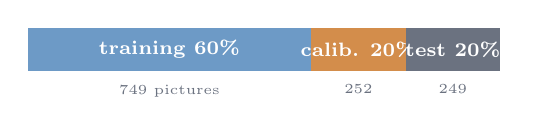
\begin{tikzpicture}
\fill[agent!70] (0,0) rectangle (3.6,0.55) node[midway,text=white,font=\scriptsize\bfseries]{training 60\%};
\fill[risk!80] (3.6,0) rectangle (4.8,0.55) node[midway,text=white,font=\scriptsize\bfseries]{calib. 20\%};
\fill[muted] (4.8,0) rectangle (6.0,0.55) node[midway,text=white,font=\scriptsize\bfseries]{test 20\%};
\node[font=\tiny,text=muted,anchor=north] at (1.8,-0.05) {749 pictures};
\node[font=\tiny,text=muted,anchor=north] at (4.2,-0.05) {252};
\node[font=\tiny,text=muted,anchor=north] at (5.4,-0.05) {249};
\end{tikzpicture}\par\vspace{8pt}
\small
\begin{itemize}\setlength\itemsep{3pt}
\item \textbf{Training books} $\to$ learn the mappings (\emph{weights}).
\item \textbf{Calibration books} $\to$ choose the cut-off $\hat\lambda$.
\item \textbf{Test books} $\to$ only to measure.
\item Repeated on \textbf{200} new random splits, so no result rests on one lucky split.
\end{itemize}
\column{0.48\textwidth}
\textbf{\color{navy}EVERY picture}\par\vspace{6pt}
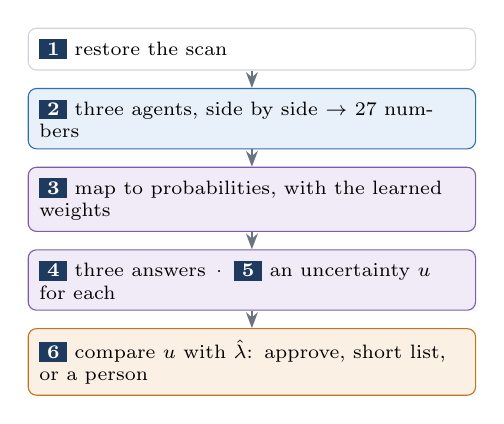
\begin{tikzpicture}[st/.style={box,minimum width=5.6cm,align=left,text width=5.4cm,font=\scriptsize},node distance=2.2mm]
\node[st] (a) {\stepn{1} restore the scan};
\node[st,draw=agent,fill=agentbg,below=of a] (b) {\stepn{2} three agents, side by side $\to$ 27 numbers};
\node[st,draw=mapc,fill=mapbg,below=of b] (c) {\stepn{3} map to probabilities, with the learned weights};
\node[st,draw=mapc,fill=mapbg,below=of c] (d) {\stepn{4} three answers \,·\, \stepn{5} an uncertainty $u$ for each};
\node[st,draw=risk,fill=riskbg,below=of d] (e) {\stepn{6} compare $u$ with $\hat\lambda$: approve, short list, or a person};
\foreach \x/\y in {a/b,b/c,c/d,d/e} \draw[arr] (\x)--(\y);
\end{tikzpicture}
\end{columns}
\note{Two phases. Once, before use: on training books the mappings are learned, on calibration books the cut-off is chosen, test books are only used to measure, and the whole thing is redone on 200 random splits. Then every new picture goes through the same six steps.}
\end{frame}

\begin{frame}{Step \stepn{3} \,·\, From an agent's numbers to a probability}
\begin{columns}[T,onlytextwidth]
\column{0.50\textwidth}
\begin{defbox}{Logistic regression (learned on training books)}
Each number gets a \textbf{weight}: how much it counts as evidence for ``scene''. Add them up with a \textbf{bias}, then squeeze the sum into 0--1:\\[2pt]
\centering$p = \dfrac{1}{1 + e^{-(\text{bias} + \sum \text{weight}\times\text{number})}}$
\end{defbox}\vspace{2pt}
\begin{exbox}
Object finder: $0.41 + 3.52\times0.972 + 2.40\times0.013 = 3.86 \to p = \mathbf{0.98}$\\
Scene matcher: sum $2.72 \to \mathbf{0.94}$\quad Describer: sum $4.55 \to \mathbf{0.99}$
\end{exbox}
\vspace{1pt}{\scriptsize Sheet music: ``no scene'' 0.89 $\to 2.01 - 2.83\times0.89 = -0.51 \to p = 0.38$.}
\column{0.47\textwidth}
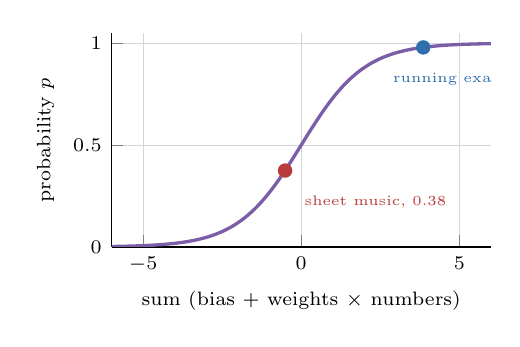
\begin{tikzpicture}
\begin{axis}[width=6.4cm,height=4.3cm,xmin=-6,xmax=6,ymin=0,ymax=1.05,
  xlabel={\scriptsize sum (bias + weights $\times$ numbers)},ylabel={\scriptsize probability $p$},
  x tick label style={font=\scriptsize},y tick label style={font=\scriptsize},axis lines*=left,grid=major,grid style={line}]
\addplot[mapc,very thick,domain=-6:6,samples=120] {1/(1+exp(-x))};
\addplot[only marks,mark=*,mark size=2.4pt,agent] coordinates {(3.86,0.979)};
\addplot[only marks,mark=*,mark size=2.4pt,pers] coordinates {(-0.51,0.375)};
\node[font=\tiny,anchor=north west,text=agent] at (axis cs:2.6,0.9) {running example, 0.98};
\node[font=\tiny,anchor=north west,text=pers] at (axis cs:-0.2,0.3) {sheet music, 0.38};
\end{axis}
\end{tikzpicture}\par
\footnotesize Learned weights, object finder: person $+3.52$, animal $+2.40$, text $-0.18$. A person counts strongly towards ``scene''; text slightly against.
\end{columns}
\note{Step three. Each agent's numbers go into a logistic regression learned on the training books: each number has a weight, we add them with a bias and squeeze the sum into a probability with the S-curve. For our picture the object finder's sum is 3.86, a probability of 0.98. A page of sheet music gets a strong no-scene score and ends at 0.38.}
\end{frame}

\begin{frame}{Step \stepn{4} \,·\, Three answers for every picture}
\begin{columns}[T,onlytextwidth]
\column{0.32\textwidth}
\begin{defbox}{Scene at all (first level)}
$p = 0.6\,p_{\text{obj}} + 0.2\,p_{\text{scene}} + 0.2\,p_{\text{desc}}$\\[4pt]
$\phantom{p} = 0.6{\times}0.98 + 0.2{\times}0.94$\\
$\phantom{p = } + 0.2{\times}0.99$\\[2pt]
$\phantom{p} = \mathbf{0.97}$ $\to$ \yes{scene}\\[4pt]
{\scriptsize Learned weights (0.43 / 0.24 / 0.33) give the same results.}
\end{defbox}
\column{0.33\textwidth}
\begin{defbox}{Scene class}
One learned mapping of all 27 numbers $\to$ six probabilities:\par
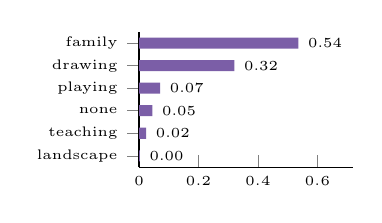
\begin{tikzpicture}
\begin{axis}[xbar,width=4.3cm,height=3.3cm,every node near coord/.append style={anchor=west},xmin=0,xmax=0.72,bar width=4pt,
  symbolic y coords={landscape,teaching,none,playing,drawing,family},ytick=data,
  y tick label style={font=\tiny},x tick label style={font=\tiny},nodes near coords,nodes near coords style={font=\tiny},
  axis lines*=left,enlarge y limits=0.1]
\addplot[fill=mapc,draw=none,point meta=explicit symbolic] coordinates {(0.536,family) [0.54] (0.321,drawing) [0.32] (0.071,playing) [0.07] (0.045,none) [0.05] (0.024,teaching) [0.02] (0.003,landscape) [0.00]};
\end{axis}
\end{tikzpicture}\par
answer: \textbf{family} (the human label)
\end{defbox}
\column{0.32\textwidth}
\begin{defbox}{Object classes}
For each class: the mean of the three agents' probabilities.\par
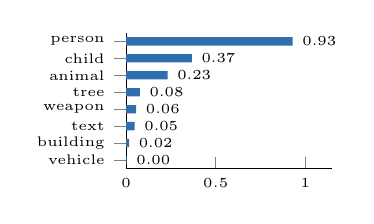
\begin{tikzpicture}
\begin{axis}[xbar,width=4.2cm,height=3.3cm,every node near coord/.append style={anchor=west},xmin=0,xmax=1.15,bar width=3pt,
  symbolic y coords={vehicle,building,text,weapon,tree,animal,child,person},ytick=data,
  y tick label style={font=\tiny},x tick label style={font=\tiny},nodes near coords,nodes near coords style={font=\tiny},
  axis lines*=left,enlarge y limits=0.07]
\addplot[fill=agent,draw=none,point meta=explicit symbolic] coordinates {(0.929,person) [0.93] (0.366,child) [0.37] (0.231,animal) [0.23] (0.077,tree) [0.08] (0.056,weapon) [0.06] (0.047,text) [0.05] (0.016,building) [0.02] (0.003,vehicle) [0.00]};
\end{axis}
\end{tikzpicture}
\end{defbox}
\end{columns}
\takeaway{Fixed weights pull rare scene classes into ``drawing'' (here they would answer drawing, 0.59). Learned, the system answers family.}
\note{Step four: three answers. Scene at all combines the three probabilities with fixed weights; learned weights give the same result. Scene class uses one learned mapping of all 27 numbers; here it says family with 0.54, which is right, while fixed weights would have said drawing. Objects: the mean of the three agents per class.}
\end{frame}

\begin{frame}{Step \stepn{5} \,·\, How unsure is each answer?}
\begin{columns}[T,onlytextwidth]
\column{0.52\textwidth}
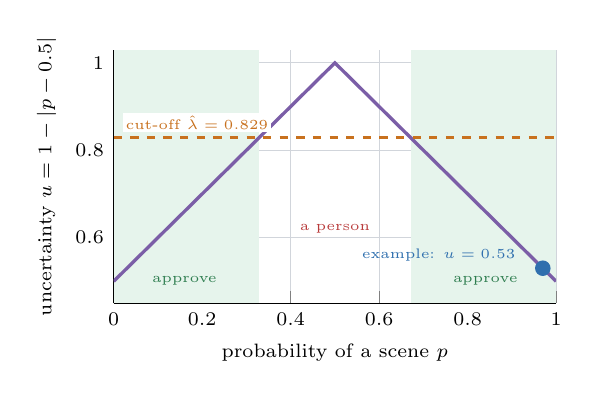
\begin{tikzpicture}
\begin{axis}[width=7.2cm,height=4.8cm,xmin=0,xmax=1,ymin=0.45,ymax=1.03,
  xlabel={\scriptsize probability of a scene $p$},ylabel={\scriptsize uncertainty $u = 1 - |p - 0.5|$},
  x tick label style={font=\scriptsize},y tick label style={font=\scriptsize},axis lines*=left,grid=major,grid style={line}]
\fill[okbg] (axis cs:0,0.45) rectangle (axis cs:0.329,1.03);
\fill[okbg] (axis cs:0.671,0.45) rectangle (axis cs:1,1.03);
\addplot[mapc,very thick,domain=0:1,samples=101] {1-abs(x-0.5)};
\addplot[risk,thick,dashed,domain=0:1] {0.829};
\addplot[only marks,mark=*,mark size=2.6pt,agent] coordinates {(0.97,0.53)};
\node[font=\tiny,text=agent,anchor=east] at (axis cs:0.93,0.56) {example: $u = 0.53$};
\node[font=\tiny,text=risk,fill=white,inner sep=1pt,anchor=south west] at (axis cs:0.02,0.84) {cut-off $\hat\lambda = 0.829$};
\node[font=\tiny,text=okc] at (axis cs:0.16,0.5) {approve};
\node[font=\tiny,text=okc] at (axis cs:0.84,0.5) {approve};
\node[font=\tiny,text=pers] at (axis cs:0.5,0.62) {a person};
\end{axis}
\end{tikzpicture}
\column{0.45\textwidth}
\begin{defbox}{Scene at all}
$u = 1 - |p - 0.5|$: highest at a coin flip ($p = 0.5$), lowest when the system is sure.
\end{defbox}\vspace{3pt}
\begin{defbox}{Scene class}
$u = 1 - $ (the largest of the six probabilities). Example: $1 - 0.54 = 0.46$.
\end{defbox}\vspace{3pt}
\begin{defbox}{Objects}
No single $u$: classes above a threshold $t$ form a \textbf{short list} for a person to confirm.
\end{defbox}
\end{columns}
\note{Step five turns each answer into an uncertainty. For scene at all it is one minus the distance from 0.5. The green zones are the probabilities that will be approved at the cut-off we will choose next. Our picture, p = 0.97, sits deep in the green. For the scene class it is one minus the largest probability. Objects become a short list.}
\end{frame}

\begin{frame}{Step \stepn{6} \,·\, Choosing the cut-off: the idea}
\centering
{\scriptsize\color{muted}Calibration pictures, sorted by their uncertainty $u$}\par\vspace{12pt}
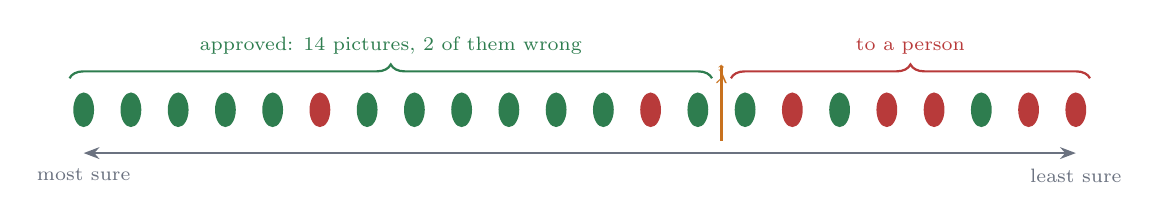
\begin{tikzpicture}[x=0.6cm]
\foreach \k/\c in {0/okc,1/okc,2/okc,3/okc,4/okc,5/pers,6/okc,7/okc,8/okc,9/okc,10/okc,11/okc,12/pers,13/okc,14/okc,15/pers,16/okc,17/pers,18/pers,19/okc,20/pers,21/pers}{
  \fill[\c] (\k,0) circle (0.22);}
\draw[<->,thick,muted] (0,-0.55) -- (21,-0.55) node[pos=0,below=2pt,font=\scriptsize]{most sure} node[pos=1,below=2pt,font=\scriptsize]{least sure};
\draw[risk,very thick] (13.5,0.55) -- (13.5,-0.4) node[above=17pt,font=\scriptsize\bfseries,text=risk]{$\hat\lambda$};
\draw[decorate,decoration={brace,amplitude=5pt},thick,okc] (-0.3,0.4)--(13.3,0.4) node[midway,above=5pt,font=\scriptsize,text=okc]{approved: 14 pictures, 2 of them wrong};
\draw[decorate,decoration={brace,amplitude=5pt},thick,pers] (13.7,0.4)--(21.3,0.4) node[midway,above=5pt,font=\scriptsize,text=pers]{to a person};
\end{tikzpicture}
\par\vspace{6pt}{\scriptsize\color{muted}Illustration with 22 pictures: \tikz\fill[okc] circle (0.1); answer right \quad \tikz\fill[pers] circle (0.1); answer wrong}\par\vspace{8pt}
\begin{columns}[T,onlytextwidth]
\column{0.48\textwidth}
\begin{enumerate}\small\setlength\itemsep{3pt}
\item Move the cut-off $\lambda$ from left to right.
\item Count the pictures that would be \textbf{approved and wrong}.
\item Stop at the last position where that count is still within the promise (with a small safety margin).
\end{enumerate}
\column{0.48\textwidth}
\begin{defbox}{The rule (conformal risk control)}
$\hat R(\lambda)$ = share approved and wrong\\[2pt]
$\hat\lambda = \max\{\lambda : \tfrac{n}{n+1}\hat R(\lambda) + \tfrac{1}{n+1} \le \alpha\}$
\end{defbox}
\end{columns}
\note{Step six, the risk promise. Sort the calibration pictures from most sure to least sure. Move the cut-off to the right: every step approves one more picture. Count how many approved pictures are wrong. Stop at the last position where that share is still within alpha, after a small allowance for having a finite calibration set. That is the whole method.}
\end{frame}

\begin{frame}{Step \stepn{6} \,·\, Choosing the cut-off: worked out}
\begin{columns}[c,onlytextwidth]
\column{0.56\textwidth}
\centering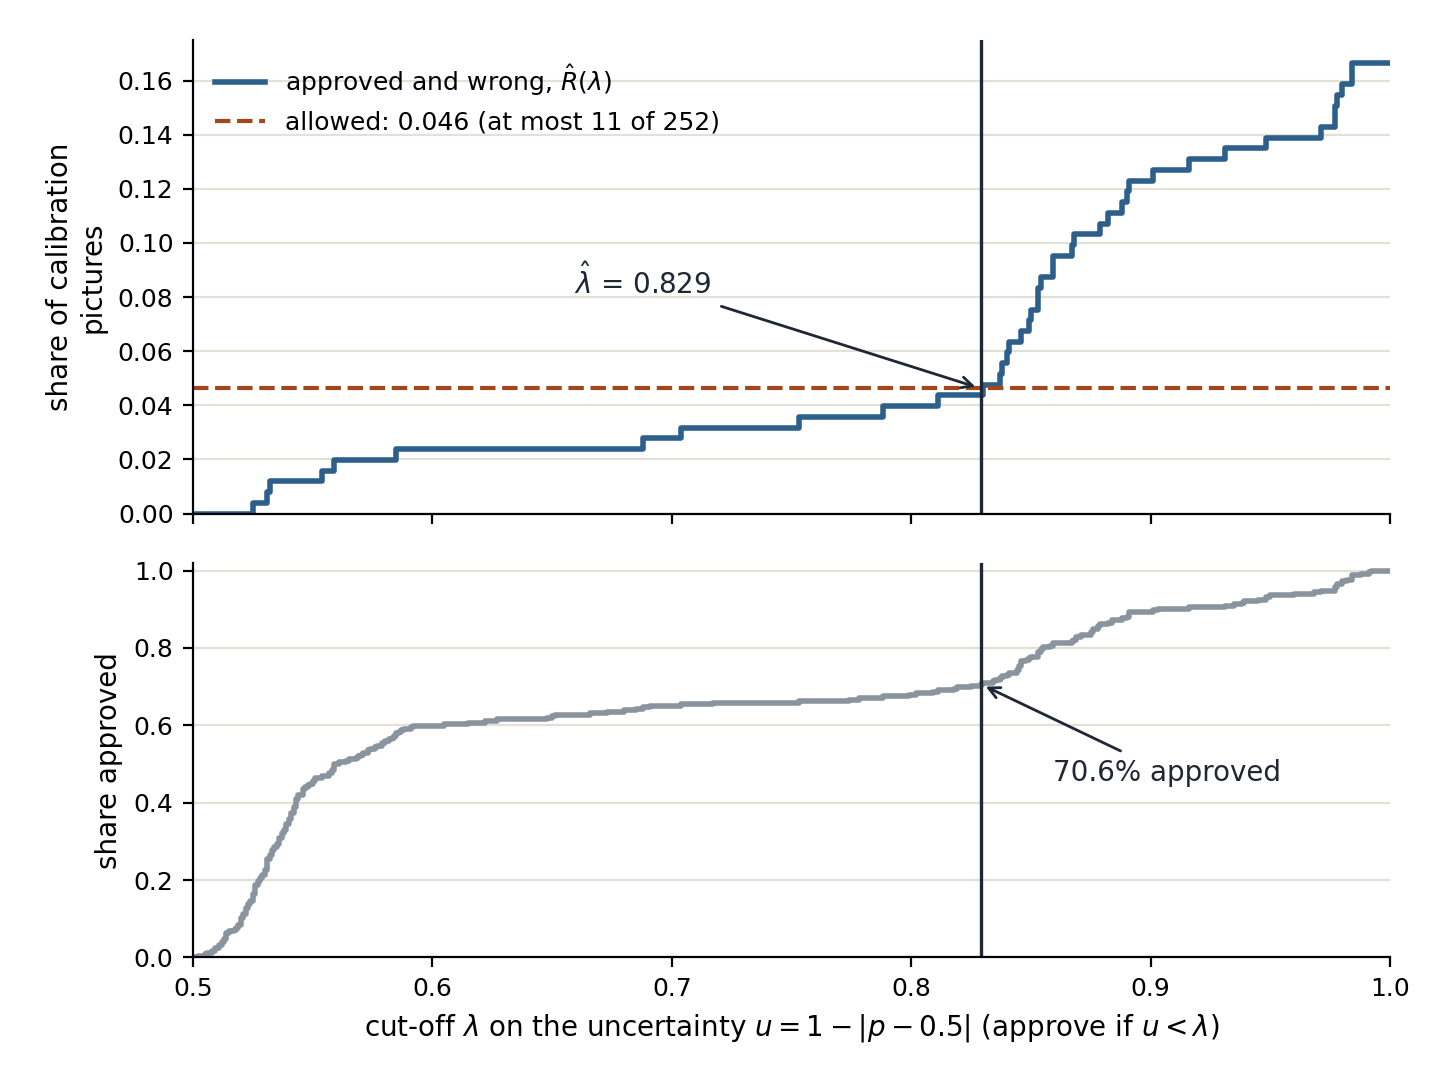
\includegraphics[width=\linewidth]{crc_cutoff_curve.png}
\column{0.42\textwidth}
\renewcommand{\defboxfont}{\scriptsize}
\begin{exbox}[fontupper=\footnotesize\raggedright]
$n = 252$ calibration pictures, $\alpha = 0.05$\\[2pt]
allowance $= 1/253 \approx 0.004$\\
$\to$ at most \textbf{11 of 252} approved and wrong\\[3pt]
largest safe cut-off: $\hat\lambda = \mathbf{0.829}$\\
$\to$ approve if $p$ is more than 0.171 from 0.5\\[3pt]
On the 249 test pictures: \yes{70.7\%} approved, real risk \yes{0.036}
\end{exbox}\vspace{4pt}
\begin{defbox}{What is promised, and what is not}
At most 5 in 100 of \emph{all} pictures approved and wrong, \textbf{on average}, for new pictures like the calibration pictures. Not the error rate among the approved; not every batch.
\end{defbox}
\end{columns}
\note{Here is the real curve. Top: the share approved and wrong rises with lambda; the dashed line is the limit, 11 of 252 pictures. The largest lambda below the line is 0.829. Bottom: that approves about 71 percent. On the test pictures the real risk was 0.036. The promise holds on average and only for pictures like the calibration pictures, which matters later.}
\end{frame}

\begin{frame}{Following one picture all the way through}
\begin{columns}[T,onlytextwidth]
\column{0.29\textwidth}
\centering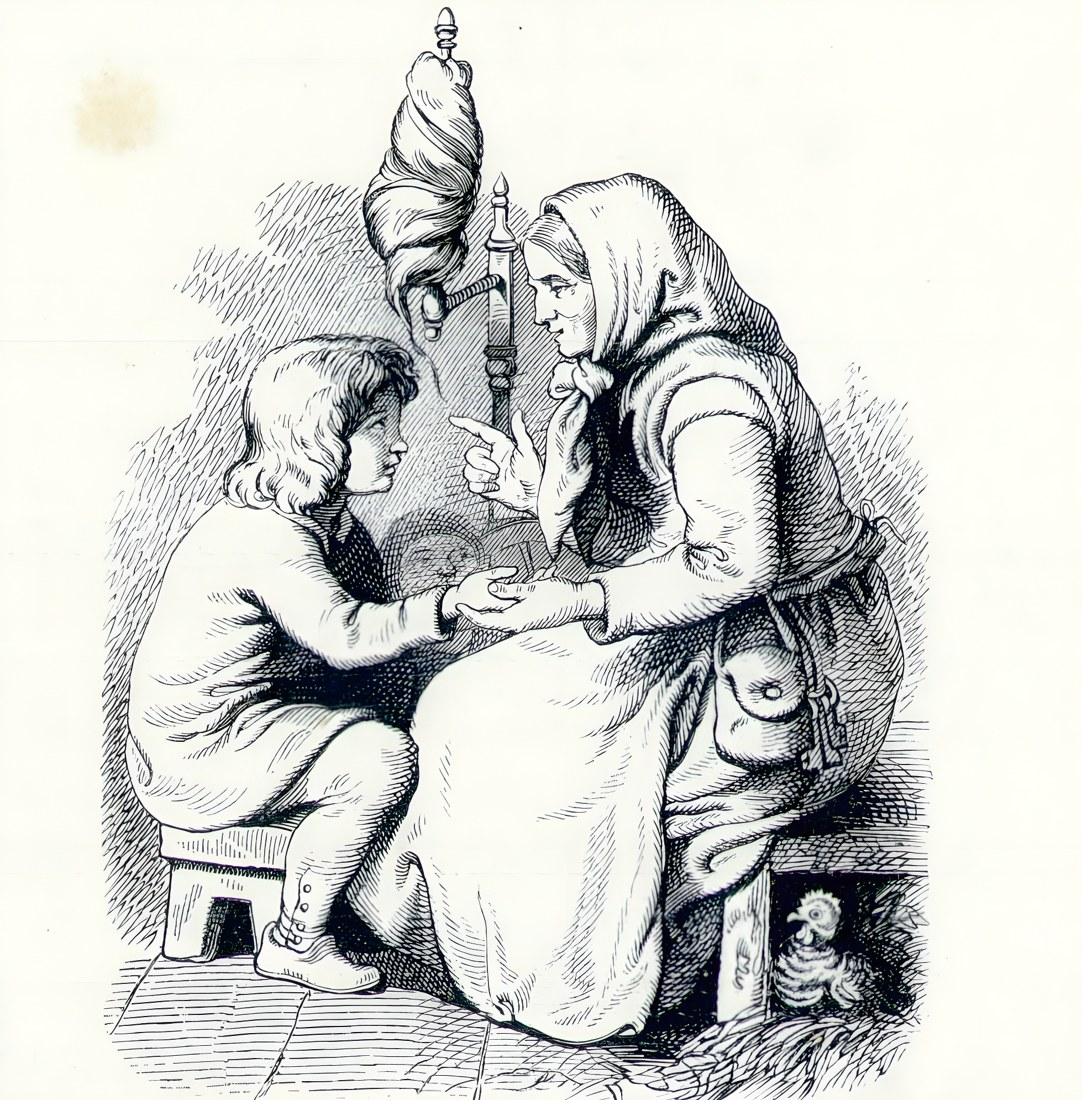
\includegraphics[height=4.1cm]{running_example.jpg}\par
{\scriptsize An old woman at her spindle talking to a boy; a small hen under the bench.\\Human label: family; person, child.}
\column{0.68\textwidth}
\small
\renewcommand{\arraystretch}{1.35}
\begin{tabularx}{\linewidth}{@{}>{\bfseries}l X l@{}}
\toprule
Answer & What the system computes & Decision\\
\midrule
Scene at all & $p = 0.97$, $u = 0.53 < \hat\lambda = 0.829$ & \yes{approved}\\
Scene class & family 0.54 (drawing 0.32); $u = 0.46 > 0.26$ & \no{a person}\\
Objects & person 0.93, child 0.37, animal 0.23; list $\ge 0.088$ & \no{person confirms}\\
\bottomrule
\end{tabularx}
\vspace{4pt}
\begin{keybox}
The system is sure there is a scene, unsure which one, and lists \textbf{person, child, animal}. The animal is the hen, which the human annotator did not box: the short list was right where the label was incomplete.
\end{keybox}
\end{columns}
\note{One picture through the whole system. Scene at all: 0.97, approved automatically. Scene class: family is right, but with 0.54 it is not sure enough, so a person decides. Objects: the list is person, child and animal; a person confirms it. The animal is the hen, which the annotator did not even box.}
\end{frame}

\begin{frame}{Tier 2 \,·\, Three helpers beside the decision}
\begin{columns}[T,onlytextwidth]
\column{0.32\textwidth}
\begin{defbox}{Contradiction checker}
\textbf{Rule:} the describer names an object the object finder did not find $\to$ a flag.\\[2pt]
\textbf{Checked:} 56\% of flags name an object that is not there (68\% with the retrained finder), against 36.5\% of all claims.
\end{defbox}
\column{0.32\textwidth}
\begin{defbox}{Cross-archive linker}
\textbf{Rule:} compare picture embeddings across books; link if similarity $\geq 0.92$.\\[2pt]
\textbf{Checked:} 38 of 50 random links (76\%) are real reprints; the rest share only the style.
\end{defbox}
\column{0.32\textwidth}
\begin{defbox}{Inscription reader}
\textbf{Rule:} the text reader reads the text in the picture.\\[2pt]
\textbf{Checked:} not usable as is; of its ``real text'', only 52.5\% comes from pictures with text.
\end{defbox}
\end{columns}
\takeaway{None of them changes a decision. They add flags and links for a cataloguer, and each was checked against a person.}
\note{Tier 2 runs beside the decision on every picture. The contradiction checker finds describer claims the detector cannot confirm; the linker finds reprints across books; the inscription reader is not usable yet. They never change a decision.}
\end{frame}

% =====================================================================================================
\section{Results and meaning}

\begin{frame}{How the results were tested}
\begin{columns}[T,onlytextwidth]
\column{0.48\textwidth}
\begin{defbox}{200 redraws}
The 1,250 pictures are split by book 200 times; everything is refitted and measured each time. We report the average and the range (2.5\%--97.5\%).
\end{defbox}\vspace{3pt}
\begin{defbox}{``Established''}
A difference counts only if its \textbf{whole range} is on one side of zero. Stricter than the usual test.
\end{defbox}
\column{0.48\textwidth}
\begin{defbox}{Fixed in advance}
From September 2026 most analyses were written down and committed \emph{before} they were run; analyses added afterwards are marked as such.
\end{defbox}\vspace{3pt}
\begin{defbox}{Reproducible}
Every number comes from a script with a fixed seed; three checkers hold the thesis text to the result files. The pipeline was rerun twice from scratch.
\end{defbox}
\end{columns}
\note{Before the results, how they were tested: 200 book-disjoint splits; a difference counts only if the whole range is on one side of zero; most tests were written down before they were run; and every number is checked against its result file.}
\end{frame}

\begin{frame}{Result 1 \,·\, More pictures approved at the same promise}
\begin{columns}[c,onlytextwidth]
\column{0.56\textwidth}
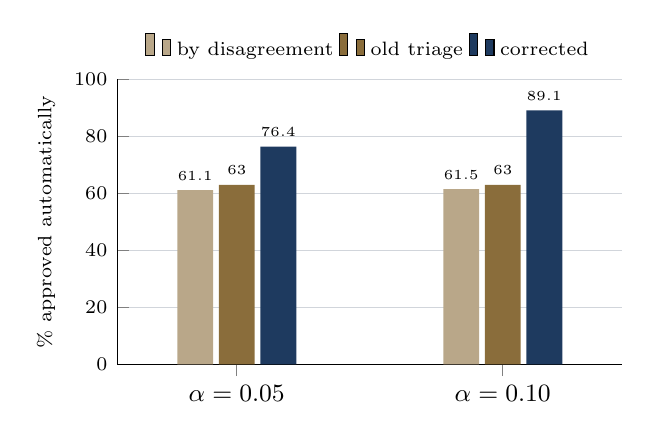
\begin{tikzpicture}
\begin{axis}[ybar,width=8cm,height=5.2cm,ymin=0,ymax=100,bar width=13pt,
  symbolic x coords={a05,a10},xtick=data,xticklabels={{$\alpha = 0.05$},{$\alpha = 0.10$}},
  x tick label style={font=\small},y tick label style={font=\scriptsize},ylabel={\scriptsize \% approved automatically},
  nodes near coords,nodes near coords style={font=\tiny},axis lines*=left,ymajorgrids,grid style={line},
  legend style={font=\scriptsize,at={(0.5,1.03)},anchor=south,legend columns=3,draw=none},enlarge x limits=0.45]
\addplot[fill=oldc!60,draw=none] coordinates {(a05,61.1) (a10,61.5)};
\addplot[fill=oldc,draw=none] coordinates {(a05,63.0) (a10,63.0)};
\addplot[fill=navy,draw=none] coordinates {(a05,76.4) (a10,89.1)};
\legend{by disagreement,old triage,corrected}
\end{axis}
\end{tikzpicture}
\column{0.42\textwidth}
\small
\begin{itemize}\setlength\itemsep{4pt}
\item Better in \textbf{199 of 200} splits.
\item Promise kept on average: real risk \textbf{0.0498} at $\alpha = 0.05$ (no margin: one split exceeds it 41.5\% of the time).
\item At the same \emph{real} error: +16 to +28 points.
\item On the archive: about \textbf{18 hours} of annotation saved at $\alpha = 0.05$.
\end{itemize}
\end{columns}
\takeaway{Inside the labelled pool, routing by confidence approves clearly more pictures than routing by disagreement, at the same promise.}
\note{The first result. At a promised 5 percent risk the corrected design approves 76 percent of pictures automatically, against 63 percent for the old triage and 61 percent by disagreement alone; better in 199 of 200 splits. The promise holds on average, but without margin.}
\end{frame}

\begin{frame}{Result 2 \,·\, On the archive the promise needs local calibration}
\begin{columns}[c,onlytextwidth]
\column{0.56\textwidth}
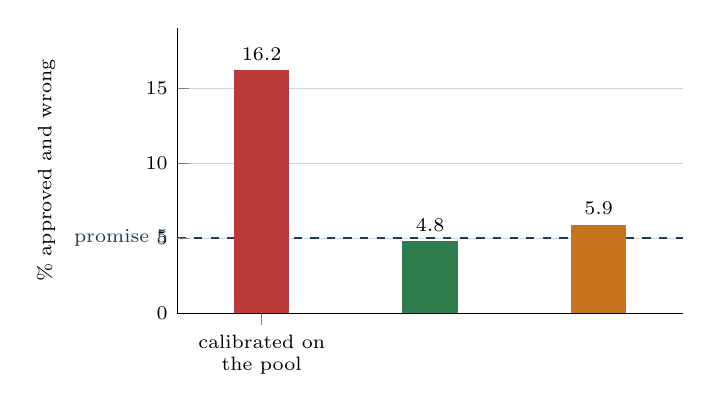
\begin{tikzpicture}
\begin{axis}[ybar,width=8cm,height=5.2cm,ymin=0,ymax=19,bar width=20pt,
  symbolic x coords={a,b,c},xtick=data,
  xticklabels={{calibrated on\\the pool},{one definition,\\archive calib.},{same, on 294\\new pictures}},
  x tick label style={font=\scriptsize,align=center},y tick label style={font=\scriptsize},ylabel={\scriptsize \% approved and wrong},
  nodes near coords,nodes near coords style={font=\scriptsize},axis lines*=left,ymajorgrids,grid style={line},enlarge x limits=0.25,
  bar shift=0pt,extra y ticks={5},extra y tick labels={\color{navy}promise 5},extra y tick style={grid=major,grid style={navy,dashed,thick},tick label style={font=\tiny}}]
\addplot[fill=pers,draw=none] coordinates {(a,16.2)};
\addplot[fill=okc,draw=none] coordinates {(b,4.8)};
\addplot[fill=risk,draw=none] coordinates {(c,5.9)};
\end{axis}
\end{tikzpicture}
\par{\scriptsize\color{muted}Middle bar: an analysis added after the test. Right bar: 5.4--5.9\% depending on the measure, test fixed in advance.}
\column{0.42\textwidth}
\small
\begin{itemize}\setlength\itemsep{4pt}
\item 400 pictures drawn at random from the archive (test fixed before labelling): the promise \no{fails}, 16.2\%.
\item Two causes: the labels mixed \textbf{two definitions} of a scene, and the pool was \textbf{not a random sample}.
\item One definition + calibration on archive pictures: just above the promise, at about \textbf{80\%} approved.
\end{itemize}
\end{columns}
\takeaway{The promise transfers only to pictures like the calibration pictures. Calibrate on a random sample of the collection itself.}
\note{The second result is the honest one. On 400 random archive pictures, with the cut-off from the labelled pool, the promise fails: 16 percent approved and wrong. Two causes: two definitions of a scene in the labels, and a pool that was not random. With one definition and calibration on archive pictures, the risk comes to just above 5 percent on new pictures, at 80 percent approved.}
\end{frame}

\begin{frame}{Result 3 \,·\, Object and scene classes}
\begin{columns}[T,onlytextwidth]
\column{0.48\textwidth}
\begin{defbox}{8 object classes (300 hand-labelled pictures)}
\begin{itemize}\setlength\itemsep{2pt}
\item The agents rank presence well: mean AUROC \textbf{0.903} (old detector 0.624, a linear probe 0.838).
\item A promise on missed objects: a list of \textbf{2.8 classes} per picture that misses 9.2\% of a picture's objects, as promised; about 1.6 wrong classes to strike out.
\end{itemize}
\end{defbox}
\column{0.48\textwidth}
\begin{defbox}{5 scene classes + no scene (992 pictures)}
\begin{itemize}\setlength\itemsep{2pt}
\item Balanced accuracy: fixed weights 0.401, describer alone 0.507, \textbf{learned 0.544}.
\item Family, playing, landscape found in 27--62\% of cases.
\item At a 5\% promise only ``no scene'' and ``drawing'' are approved (69.1\% of pictures); specific classes go to a person.
\item Random archive pictures: \no{0.351}.
\end{itemize}
\end{defbox}
\end{columns}
\takeaway{Objects: a reliable short list. Scene classes: the system shortlists, a person decides. One vision-language model alone is about as good as the combination.}
\note{On the class tasks the system is useful for objects: a short list of about three classes that misses less than one object in ten. For scene classes it can shortlist but not decide: only no scene and drawing can be approved, and on random archive pictures the balanced accuracy drops to 0.35. And the describer alone is about as good as the combination.}
\end{frame}

\begin{frame}{Result 4 \,·\, People do not fully agree either}
\begin{columns}[c,onlytextwidth]
\column{0.52\textwidth}
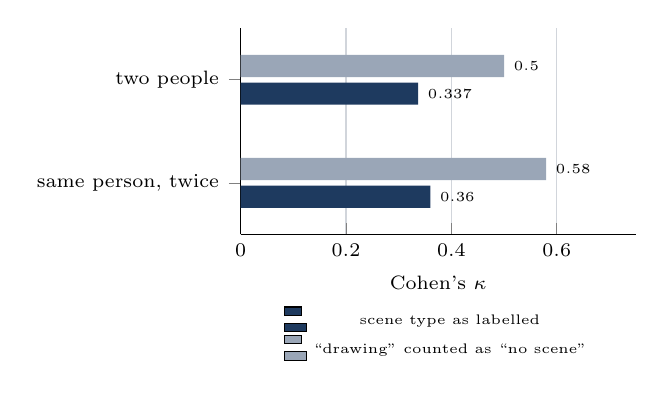
\begin{tikzpicture}
\begin{axis}[xbar,width=6.6cm,height=4.2cm,xmin=0,xmax=0.75,bar width=8pt,
  symbolic y coords={{same person, twice},{two people}},ytick=data,
  y tick label style={font=\scriptsize},x tick label style={font=\scriptsize},xlabel={\scriptsize Cohen's $\kappa$},
  nodes near coords,nodes near coords style={font=\tiny},axis lines*=left,xmajorgrids,grid style={line},
  legend style={font=\tiny,at={(0.5,-0.32)},anchor=north,legend columns=1,draw=none},enlarge y limits=0.5]
\addplot[fill=navy,draw=none] coordinates {(0.337,{two people}) (0.36,{same person, twice})};
\addplot[fill=navy!45,draw=none] coordinates {(0.50,{two people}) (0.58,{same person, twice})};
\legend{scene type as labelled,``drawing'' counted as ``no scene''}
\end{axis}
\end{tikzpicture}
\column{0.45\textwidth}
\small
\begin{itemize}\setlength\itemsep{4pt}
\item Two raters on 124 pictures: $\kappa = 0.337$.
\item One rater, 143 pictures a second time: $\kappa = 0.36$.
\item Most disagreement is about ``drawing''.
\end{itemize}
\begin{keybox}
Scene categories are interpretations, not facts. This limits what any system can reach and how its errors can be counted.
\end{keybox}
\end{columns}
\note{People agree only moderately on scene types: kappa 0.34 between two raters and 0.36 for the same rater twice. Most of it is about drawing. This sets a ceiling for any system and is why the thesis reports per definition.}
\end{frame}

\begin{frame}{What is new: the contributions}
\footnotesize
\renewcommand{\arraystretch}{1.3}
\begin{tabularx}{\textwidth}{@{}c >{\raggedright\arraybackslash}p{4.6cm} >{\raggedright\arraybackslash}X@{}}
\toprule
& \textbf{Contribution} & \textbf{Evidence}\\
\midrule
\textbf{\color{navy}1} & \textbf{Disagreement does not find errors} better than confidence, and why & Fixed in advance: 0.378 against 0.825; within task 0.78 / 0.82 against 0.84 / 0.83; 149 of 199 errors shared\\
\textbf{\color{navy}2} & \textbf{An audit of what an uncertainty score measures} & The deployed four signals were two measurements and eight states\\
\textbf{\color{navy}3} & \textbf{Pseudo-label scores hide failure}, traced to the teacher & 0.768 against the teacher, 0.146 against people; 126 of 128 misses never labelled; better teacher 0.123 $\to$ 0.210\\
\textbf{\color{navy}4} & \textbf{A corrected design with a risk promise} & 76.4\% approved at 5\% against 63.0\% (199 of 200 redraws); object list of 2.8 classes, 9.2\% missed\\
\textbf{\color{navy}5} & \textbf{The promise tested where it is used} & Random archive pictures: 16.2\% with pool calibration; 5.4--5.9\% at 80\% approved with archive calibration\\
\bottomrule
\end{tabularx}
\takeaway{The result is knowledge about \emph{when} an automatic answer can be trusted: route by confidence, calibrate on the collection itself, promise what each task needs.}
\note{If I am asked what I improved: five contributions. One, a tested negative answer to a common assumption, with the reason. Two, an audit method that showed what the deployed uncertainty score really measured. Three, the finding that pseudo-label scores hide failure, traced to the teacher. Four, a corrected design that follows from these findings and approves clearly more at the same promise. Five, the promise tested where it is used, on random archive pictures, with a practical rule: calibrate on the collection itself.}
\end{frame}

\begin{frame}{What the thesis establishes, and what it does not claim}
\begin{columns}[T,onlytextwidth]
\column{0.48\textwidth}
\begin{defbox}[colframe=okc,colbacktitle=okbg,coltitle=okc]{Established}
\begin{itemize}\setlength\itemsep{2pt}
\item Disagreement never ranks errors better than confidence here; most errors are shared.
\item The first design's signals were two measurements (8 states).
\item Pseudo-label scores hide a collapse (0.768 vs 0.146).
\item Confidence routing approves more at the same promise (pool).
\item The promise holds on new pictures only when calibrated on similar pictures.
\end{itemize}
\end{defbox}
\column{0.48\textwidth}
\begin{defbox}[colframe=pers,colbacktitle=persbg,coltitle=pers]{Not claimed}
\begin{itemize}\setlength\itemsep{2pt}
\item That disagreement beats confidence.
\item A guarantee for every batch: the promise is an average.
\item That the accuracy gains transfer to other label sources ($\kappa = 0.41$ between sources).
\item Automatic scene classes: they need a person.
\item That several agents clearly beat one.
\end{itemize}
\end{defbox}
\end{columns}
\note{What I claim and what I do not. Established: disagreement does not beat confidence; the old signals were two measurements; pseudo-label scores can hide a collapse; confidence routing approves more; and the promise needs similar calibration pictures. Not claimed: a per-batch guarantee, transfer to other label sources, automatic scene classes, or that several agents beat one.}
\end{frame}

\begin{frame}{Limitations and next steps}
\begin{columns}[T,onlytextwidth]
\column{0.48\textwidth}
\begin{defbox}{Limitations}
\begin{itemize}\setlength\itemsep{2pt}
\item Few labelled pictures: 249 per test split, 38 without a scene; ``teaching'' has only 6.
\item The archive tests rest on one person's labels.
\item Tier 3 (paid models) designed, not run.
\item Another archive (Europeana, 24 pictures): 65.2\% of scenes missed; it does not transfer unchanged.
\end{itemize}
\end{defbox}
\column{0.48\textwidth}
\begin{defbox}{Next steps}
\begin{itemize}\setlength\itemsep{2pt}
\item Calibrate on a random, labelled sample of each new collection.
\item Written definitions for the scene classes, and a second rater.
\item A promise per class or per batch (e.g.\ Learn then Test).
\item Before trusting disagreement anywhere: check the agents really differ (effective rank $\geq 2$).
\end{itemize}
\end{defbox}
\end{columns}
\note{The limitations are mostly about labels: few test pictures, one person's labels on the archive, and scene classes without written definitions. The transfer pilot on Europeana shows the method does not carry over unchanged. Next steps follow directly: calibrate locally, define classes, and check that agents differ before relying on disagreement.}
\end{frame}

\begin{frame}{Three things to remember}
\vspace{6pt}
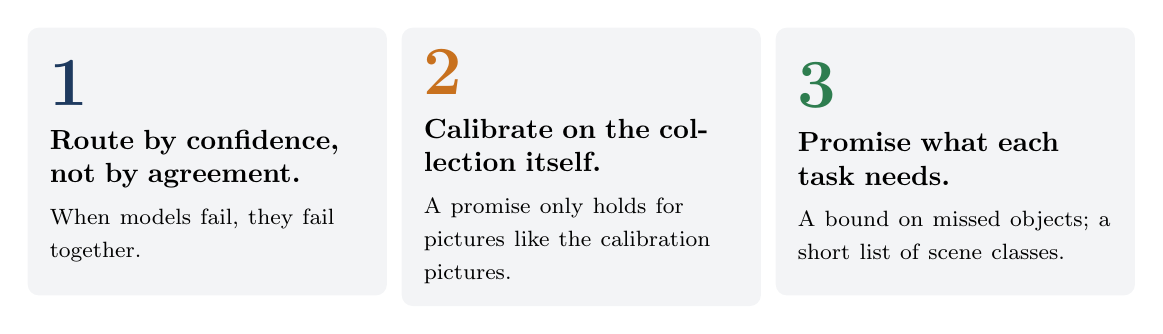
\begin{tikzpicture}[c/.style={draw=none,fill=soft,rounded corners=4pt,text width=4.0cm,minimum height=3.4cm,align=left,inner sep=8pt,anchor=north west}]
\node[c] (a) at (0,0) {{\Huge\bfseries\color{navy}1}\par\vspace{4pt}\textbf{Route by confidence, not by agreement.}\par\vspace{3pt}\footnotesize When models fail, they fail together.};
\node[c] (b) at (4.75,0) {{\Huge\bfseries\color{risk}2}\par\vspace{4pt}\textbf{Calibrate on the collection itself.}\par\vspace{3pt}\footnotesize A promise only holds for pictures like the calibration pictures.};
\node[c] (c) at (9.5,0) {{\Huge\bfseries\color{okc}3}\par\vspace{4pt}\textbf{Promise what each task needs.}\par\vspace{3pt}\footnotesize A bound on missed objects; a short list of scene classes.};
\end{tikzpicture}
\vfill
\centering{\Large\bfseries\color{navy}Thank you. Questions?}\par\vspace{4pt}
{\tiny\color{muted}Code: github.com/brhanug/Multi-Agent-Systems-For-Image-Analysis-Object-and-Complex-Scene-Detection, branch thesis-submission}
\note{Three things to remember: route by confidence, calibrate on the collection itself, and promise what each task needs. Thank you; I am happy to take questions.}
\end{frame}

% =====================================================================================================
\appendix
\section{Backup}
\begin{frame}[plain,noframenumbering]
\centering\vspace*{2.4cm}{\Huge\bfseries\color{navy}Backup slides}\par\vspace{6pt}{\small\color{muted}algorithms, the first design's cut-off, weights, practical value}
\end{frame}

\begin{frame}{Backup \,·\, ``Isn't this just a pipeline?''}
\begin{columns}[T,onlytextwidth]
\column{0.48\textwidth}
\begin{defbox}{The short answer}
The pipeline is the \textbf{instrument}. The thesis is a set of \textbf{tested claims}, each with a test fixed before it was run, a measure against people, and a result that could have gone either way:
\begin{itemize}\setlength\itemsep{1pt}
\item the main hypothesis was \textbf{rejected} (RQ1);
\item the first design was \textbf{audited and replaced} because of what the tests showed;
\item the risk promise was \textbf{tested off the labelled pool} and failed before it was repaired.
\end{itemize}
A pipeline project reports that its system works. This thesis reports where it does not, and why.
\end{defbox}
\column{0.48\textwidth}
\begin{defbox}{What makes it research}
\begin{itemize}\setlength\itemsep{2pt}
\item A hypothesis from the literature (committee and ensemble disagreement), tested on a new kind of data.
\item Pre-registered tests; book-disjoint splits; 200 redraws; a stated rule for ``established''.
\item Negative results reported and explained (shared errors, eight states, teacher's missing classes).
\item Every figure held to its result file by scripted checks; code public.
\end{itemize}
\end{defbox}
\end{columns}
\note{If someone says I only built a pipeline: the pipeline is the instrument. The research is the hypothesis it was built to test, the tests fixed in advance, and the results, including the negative ones: the main hypothesis was rejected, the first design was audited and replaced, and the promise failed on the archive before it was repaired. A pipeline project would report that its system works; this thesis reports where it does not and why.}
\end{frame}

\begin{frame}{Backup \,·\, Algorithm 1: learning the mappings (once, training books)}
\begin{columns}[T,onlytextwidth]
\column{0.55\textwidth}
\begin{defbox}{Steps}
\textbf{Input:} 749 training pictures with a human label (scene 1 / no scene 0) and each agent's numbers.
\begin{enumerate}\setlength\itemsep{2pt}
\item For each agent (object finder, scene matcher, describer):
\item \quad collect its numbers for every training picture;
\item \quad fit a logistic regression: label $\leftarrow$ its numbers;
\item \quad keep the bias and one weight per number.
\item Scene class: one multinomial regression on all 27 numbers $\to$ 6 answers.
\item Objects: per class, one regression per agent.
\end{enumerate}
\textbf{Output:} the weights, used for every picture afterwards.
\end{defbox}
\column{0.42\textwidth}
\begin{defbox}{Largest learned weights}
\textbf{Object finder:} person $+3.52$, animal $+2.40$, text $-0.18$\\[2pt]
\textbf{Scene matcher:} drawing $+2.43$, ``no scene'' $-2.83$\\[2pt]
\textbf{Describer:} person $+3.10$, animal $+2.12$, text $-0.35$
\end{defbox}\vspace{3pt}
{\footnotesize The system learns from labelled examples how much each number is evidence for each answer.}
\end{columns}
\end{frame}

\begin{frame}{Backup \,·\, Algorithm 2: deciding one picture}
\begin{defbox}{Steps (every picture)}
\textbf{Input:} a scan; the weights (Algorithm 1); the cut-offs $\hat\lambda$ (Algorithm 3).
\begin{enumerate}\setlength\itemsep{2pt}
\item Restore the scan; run the three agents $\to$ 27 numbers.
\item \textbf{Scene class:} 6 probabilities from all 27 numbers; answer = the largest; $u = 1 - $ largest; approve if $u < \hat\lambda_{\text{class}}$, else a person.
\item \textbf{Objects:} per class the mean of the 3 probabilities; list = classes $\geq t$; a person confirms the list.
\item \textbf{Scene at all:} each agent $p_k = 1 / (1 + e^{-(b_k + w_k\cdot z_k)})$; $p = 0.6\,p_1 + 0.2\,p_2 + 0.2\,p_3$; scene if $p \geq 0.5$.
\item $u = 1 - |p - 0.5|$; approve if $u < \hat\lambda$, else a person.
\end{enumerate}
\textbf{Output:} three answers, each approved or routed to a person.
\end{defbox}
\end{frame}

\begin{frame}{Backup \,·\, Algorithm 3: choosing the cut-off (once, calibration books)}
\begin{columns}[T,onlytextwidth]
\column{0.55\textwidth}
\begin{defbox}{Steps}
\textbf{Input:} $n$ calibration pictures, each with its uncertainty $u_i$ and whether its answer was wrong ($e_i = 1$) or right ($e_i = 0$); the promise $\alpha$.
\begin{enumerate}\setlength\itemsep{2pt}
\item For each candidate cut-off $\lambda$ from 0.001 to 1 (steps of 0.001):
\item \quad $\hat R(\lambda) = \tfrac1n \sum_i e_i \cdot [u_i < \lambda]$ (approved and wrong);
\item keep the largest $\lambda$ with $\tfrac{n}{n+1}\hat R(\lambda) + \tfrac{1}{n+1} \le \alpha$;
\item if none qualifies, approve nothing.
\end{enumerate}
\textbf{Output:} the cut-off $\hat\lambda$, one per answer.
\end{defbox}
\column{0.42\textwidth}
\begin{defbox}{Why it works}
Needs no assumption about the models, only that new pictures are \emph{exchangeable} with the calibration pictures (like them). This is exactly what failed on the archive with pool calibration.
\end{defbox}
\end{columns}
\end{frame}

\begin{frame}{Backup \,·\, The first design's cut-off had to fall between two of the eight rows}
\small
\renewcommand{\arraystretch}{1.12}
\begin{tabular}{@{}l r r r l@{}}
\toprule
Row $(A^{\text{object}}, A^{\text{scene}}, A^{\text{vlm}})$ & $U_{\text{SAA}}$ & $U_{\text{triage}}$ & Pictures & At $\hat\lambda = 0.372$\\
\midrule
$(1, 1, 1)$ & 0.0000 & 0.0000 & 4,154 & \yes{approved}\\
$(\tfrac23, 1, 1)$ & 0.1924 & 0.1821 & 565 & \yes{approved}\\
$(1, 0.5, 1)$ & 0.2500 & 0.2000 & 2,580 & \yes{approved}\\
$(\tfrac23, 0.5, 1)$ & 0.2097 & 0.2425 & 969 & \yes{approved}\\
$(\tfrac13, 1, 1)$ & 0.3849 & 0.3643 & 222 & \yes{approved}\\
$(\tfrac13, 0.5, 1)$ & 0.3155 & 0.3726 & 2,217 & \no{a person}\\
$(0, 0.5, 0)$ & 0.4787 & 0.5372 & 1,208 & \no{a person}\\
$(0, 1, 0)$ & 0.5774 & 0.5464 & 195 & \no{a person}\\
\bottomrule
\end{tabular}
\par\vspace{6pt}
{\footnotesize $U_{\text{SAA}}$ from Table D.3 of the thesis; $U_{\text{triage}} = 0.6\,U_{\text{SAA}} + 0.4\,(1 - \text{mean of the four signals})$. Passing 0.3726 would approve a row whose $SAA$ sits exactly on 0.5 and whose errors break the 5\% promise, so the largest safe cut-off is 0.372 (the same in 2,000 resamples).}
\end{frame}

\begin{frame}{Backup \,·\, Do the weights 0.6 / 0.2 / 0.2 matter?}
\small
\begin{columns}[T,onlytextwidth]
\column{0.56\textwidth}
\renewcommand{\arraystretch}{1.2}\footnotesize
\begin{tabular}{@{}l c c c@{}}
\toprule
Scene at all & Ranking & Wrong & Approved\\
\midrule
0.6 / 0.2 / 0.2 & 0.866 & 15.6\% & 76.4\%\\
Equal thirds & 0.865 & 15.7\% & 76.3\%\\
Learned (0.43 / 0.24 / 0.33) & 0.863 & 15.7\% & 75.6\%\\
Object finder alone & 0.852 & 15.8\% & 72.9\%\\
\bottomrule
\end{tabular}
\column{0.40\textwidth}
\begin{defbox}{Answer}
For \textbf{scene at all}: no, they give the same results; the fixed ones are kept because the archive tests were fixed with them.\\[2pt]
For \textbf{scene classes}: yes, learned 0.544 against fixed 0.401 balanced accuracy, so the system uses the learned mapping.
\end{defbox}
\end{columns}
\end{frame}

\begin{frame}{Backup \,·\, Practical value, retrieval and transfer}
\begin{columns}[T,onlytextwidth]
\column{0.32\textwidth}
\begin{defbox}{Annotation effort}
On the 12,110 pictures at $\alpha = 0.05$ the corrected design saves \textbf{18.2 hours} of full annotation, at the price of about 603 against 201 wrong labels let through (pool calibration).
\end{defbox}
\column{0.32\textwidth}
\begin{defbox}{Retrieval}
Judged by a person on 4 queries: Precision@10 \textbf{0.60} for the semantic index against 0.10 for keywords. The earlier proxy labels said 1.000.
\end{defbox}
\column{0.32\textwidth}
\begin{defbox}{Transfer (Europeana)}
24 pictures from 10 institutions: the unchanged pipeline misses \textbf{65.2\%} of scenes; its agents span about one independent direction (effective rank 1.37).
\end{defbox}
\end{columns}
\vspace{6pt}
\begin{defbox}{Speed}
Per picture on one RTX A6000: object finder 0.06\,s, describer 1.56\,s, text reader 3.23\,s. Inference is not the limit for scaling; labels are.
\end{defbox}
\end{frame}

\end{document}
